\documentclass[11pt,a4paper]{article}

\usepackage[utf8]{inputenc}
\usepackage[T1]{fontenc}
\usepackage[french]{babel}
\usepackage{geometry}
\geometry{a4paper, margin=2.2cm}
\usepackage{graphicx}
\usepackage{svg}
\svgsetup{inkscapelatex=false}
\usepackage{hyperref}
\usepackage{listings}
\usepackage{xcolor}
\usepackage{caption}
\usepackage{float}
\usepackage{placeins}

\hypersetup{
    colorlinks=true,
    linkcolor=blue,
    filecolor=magenta,
    urlcolor=cyan,
    pdftitle={Rapport DevOps - Travelo},
    pdfauthor={Adam Ait Oufkir et El Mehdi Fatahllah}
}

\definecolor{lightgray}{rgb}{0.95,0.95,0.95}
\lstset{
    backgroundcolor=\color{lightgray},
    basicstyle=\ttfamily\small,
    breaklines=true,
    frame=single,
    numbers=left,
    numbersep=5pt,
    numberstyle=\tiny\color{gray}
}

\title{
    \normalsize Institut National des Postes et Télécommunication \\
    Master Data \& IA \\
    Conteneurisation et Orchestration des Conteneurs \\
    Année universitaire 2025/2026 \\
    \vspace{1.5cm}
    \Huge \textbf{Rapport de Projet DevOps : Travelo} \\
    \Large Conteneurisation Docker, orchestration Kubernetes et observabilité
}
\author{Adam Ait Oufkir \& El Mehdi Fatahllah}
\date{}

\begin{document}

\maketitle
\thispagestyle{empty}
\vfill
\noindent\textbf{Dépôt GitHub :} \url{https://github.com/ElmehdiFATAHLLAH/travelo-app.git}
\newpage

\tableofcontents
\newpage

\section{Contexte du projet}

Travelo est une application web de réservation de vols. L'architecture applicative est composée de trois parties :
\begin{itemize}
    \item \textbf{Frontend} : application React servie par Nginx.
    \item \textbf{Backend} : API REST Spring Boot.
    \item \textbf{Base de données} : MySQL 8.
\end{itemize}

L'objectif de ce travail est de documenter le cycle DevOps complet de l'application : conteneurisation avec Docker, exécution locale avec Docker Compose, publication sur registres Docker, déploiement bonus avec Docker Swarm, puis passage vers un déploiement Kubernetes complet, isolé dans un namespace, sécurisé avec RBAC, résilient grâce aux probes et aux PodDisruptionBudgets, et observable avec Prometheus, Grafana, Loki et Promtail.

\subsection{Organisation du dépôt}

Le dépôt contient les dossiers suivants :
\begin{itemize}
    \item \texttt{k8s/base/} : manifestes Kubernetes obligatoires pour le namespace \texttt{travelo}.
    \item \texttt{k8s/monitoring/} : configuration Prometheus, Grafana, Loki et Promtail.
    \item \texttt{k8s/helm/travelo/} : chart Helm bonus.
    \item \texttt{k8s/gitops/} : exemple d'application Argo CD bonus.
    \item \texttt{skaffold.yaml} : workflow bonus Build / Deploy automatisé.
    \item \texttt{screenshots/volet1/} : captures extraites du rapport Word du Volet 1.
    \item \texttt{screenshots/generated/} : preuves d'exécution utilisées dans ce rapport.
\end{itemize}

% Fichier généré à partir de rapport_volet1_final.md et des images extraites de rapport_volet1_final.docx.
\section{Volet 1 : Conteneurisation Docker et Docker Swarm}

\textbf{Conteneurisation et Orchestration des Conteneurs}



\subsection{Introduction}

Ce rapport présente le travail réalisé dans le cadre du Volet 1 du mini-projet NeoTech, qui consiste en la conteneurisation de l'application web 3-tiers \textbf{Travelo} (React, Spring Boot, MySQL) à l'aide de Docker, ainsi que son déploiement en mode cluster avec Docker Swarm.



\subsection{1. Création du réseau Docker}

Un réseau Docker dédié est créé avec le driver bridge afin d'isoler les conteneurs et permettre leur communication par nom de service.

\begin{lstlisting}[language=bash]
docker network create --driver bridge travelo-network
\end{lstlisting}

\begin{figure}[H]
    \centering
    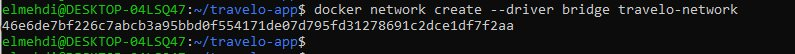
\includegraphics[width=0.95\textwidth]{./screenshots/volet1/01_creation_reseau_docker_travelo-network.png}
    \caption{Création du réseau Docker "travelo-network" avec le driver bridge}
\end{figure}

Le driver bridge est le choix le plus adapté pour une utilisation locale (single host) : il crée un réseau virtuel isolé sur la machine hôte, permettant la communication entre conteneurs via leur nom.



\subsection{2. Création du conteneur MySQL avec stockage persistant}

\subsubsection{2.a. Volume Docker pour la persistance}

Le stockage des données MySQL est rendu persistant via un volume Docker nommé, garantissant l'indépendance des données par rapport au cycle de vie du conteneur.

\begin{lstlisting}[language=bash]
docker volume create travelo_mysql_data
\end{lstlisting}

\begin{figure}[H]
    \centering
    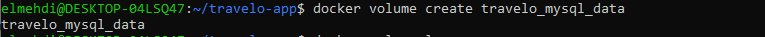
\includegraphics[width=0.95\textwidth]{./screenshots/volet1/02_creation_volume_docker_travelo_mysql_data.png}
    \caption{Création du volume Docker "travelo\_mysql\_data"}
\end{figure}

\subsubsection{2.b. Lancement du conteneur MySQL}

\begin{lstlisting}[language=bash]
docker run -d --name travelo_app --network travelo-network \
  -v travelo_mysql_data:/var/lib/mysql \
  -e MYSQL_ROOT_PASSWORD=password -e MYSQL_DATABASE=travelo_db \
  mysql:8
\end{lstlisting}

\begin{itemize}
    \item \texttt{-d} : Mode détaché
    \item \texttt{--name} : Nom du conteneur
    \item \texttt{--network} : Réseau partagé
    \item \texttt{-v} : Volume persistant
    \item \texttt{-e} : Variables d'environnement
\end{itemize}

\begin{figure}[H]
    \centering
    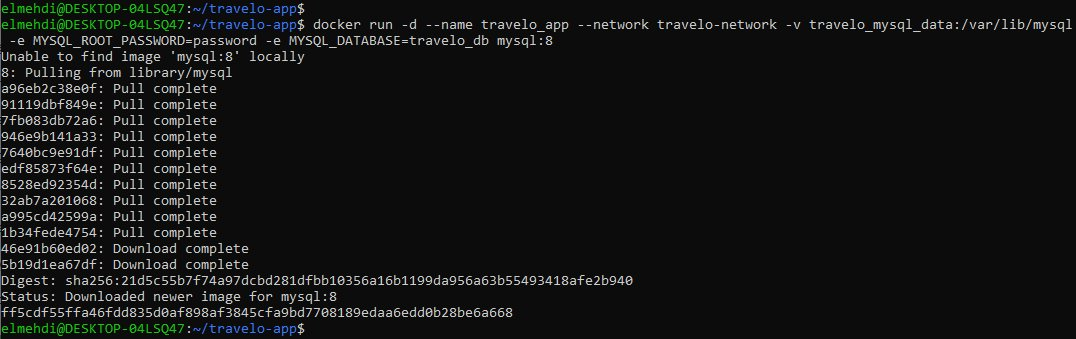
\includegraphics[width=0.95\textwidth]{./screenshots/volet1/03_lancement_conteneur_mysql_pull_demarrage.png}
    \caption{Lancement du conteneur MySQL (pull et démarrage de mysql:8)}
\end{figure}

\begin{figure}[H]
    \centering
    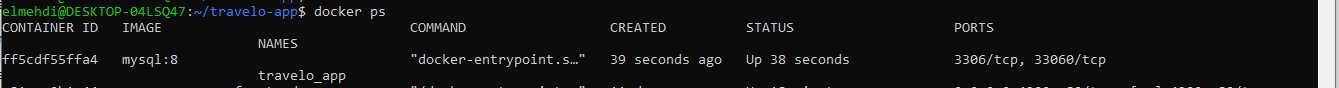
\includegraphics[width=0.95\textwidth]{./screenshots/volet1/04_docker_ps_conteneur_mysql_travelo_app_actif.png}
    \caption{\texttt{docker ps} : conteneur MySQL "travelo\_app" actif}
\end{figure}

\begin{figure}[H]
    \centering
    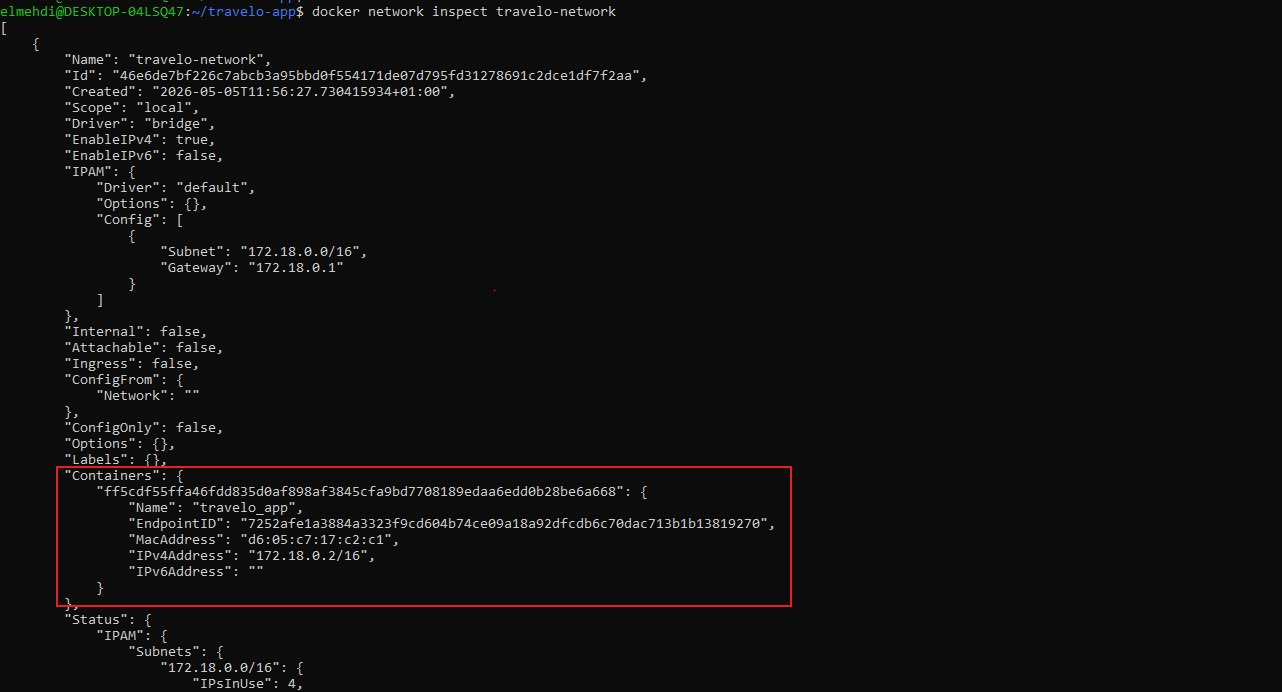
\includegraphics[width=0.95\textwidth]{./screenshots/volet1/05_inspection_reseau_travelo-network_mysql_connecte.png}
    \caption{Inspection du réseau travelo-network : conteneur MySQL connecté}
\end{figure}



\subsection{3. Dockerfile Backend – Bonnes pratiques}

\begin{figure}[H]
    \centering
    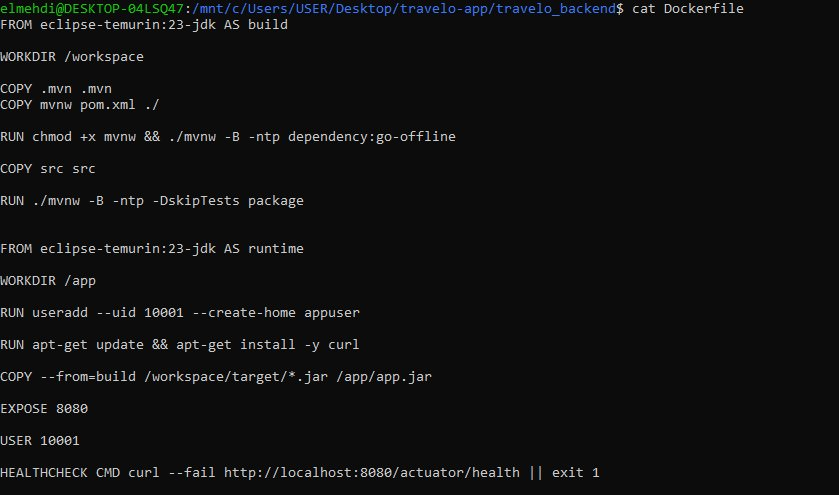
\includegraphics[width=0.95\textwidth]{./screenshots/volet1/06_dockerfile_backend_multistage_build_jdk23.png}
    \caption{Contenu du Dockerfile Backend (multi-stage build, JDK 23)}
\end{figure}



\subsection{4. Explication des bonnes pratiques}

\subsubsection{a. Multi-stage build}

Deux étapes distinctes : "build" (compilation Maven) et "runtime" (image légère). L'image finale exclut les outils de build, réduisant sa taille.

\subsubsection{b. Cache des dépendances Maven}

Copie séparée de \texttt{pom.xml} avant le code source pour exploiter le cache Docker : les dépendances ne sont retéléchargées que si \texttt{pom.xml} change.

\subsubsection{c. -DskipTests}

Les tests sont ignorés au build Docker ; ils sont exécutés séparément dans le pipeline CI/CD.

\subsubsection{d. Utilisateur non-root (UID 10001)}

Un utilisateur système \texttt{appuser} est créé pour exécuter l'application, respectant le principe du moindre privilège.

\subsubsection{e. HEALTHCHECK}

Surveillance de l'endpoint \texttt{/actuator/health} de Spring Boot pour que Docker monitore l'état de santé du conteneur.

\subsubsection{f. EXPOSE}

Documentation du port 8080 sans publication automatique sur l'hôte.



\subsection{5. Commandes Docker – Image Backend}

\subsubsection{5.a. Build de l'image}

\begin{lstlisting}[language=bash]
docker build -t travelo_backend_image .
\end{lstlisting}

\begin{figure}[H]
    \centering
    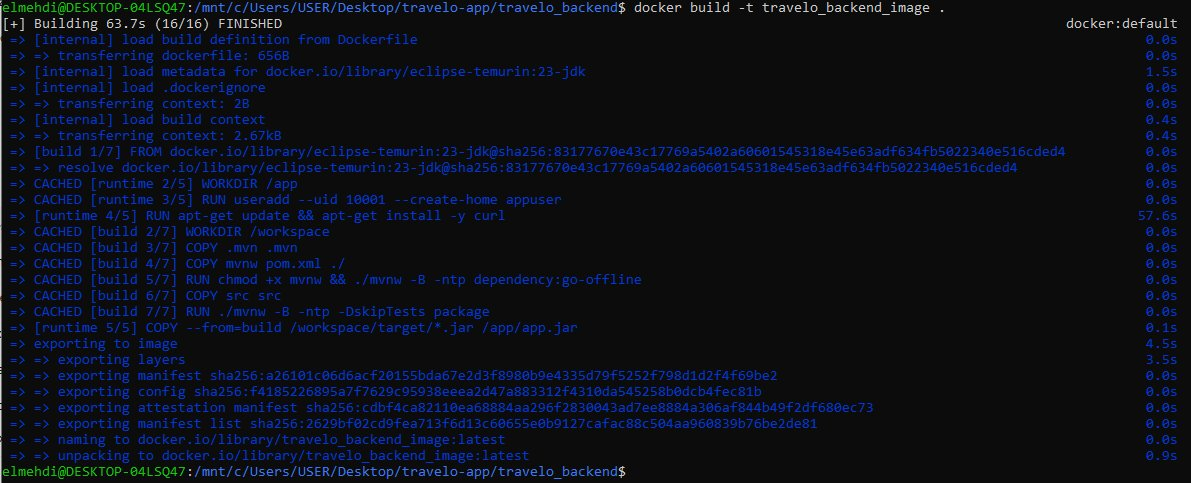
\includegraphics[width=0.95\textwidth]{./screenshots/volet1/07_build_backend_travelo_backend_image_succes.png}
    \caption{Build réussi de travelo\_backend\_image (16/16 étapes)}
\end{figure}

\begin{figure}[H]
    \centering
    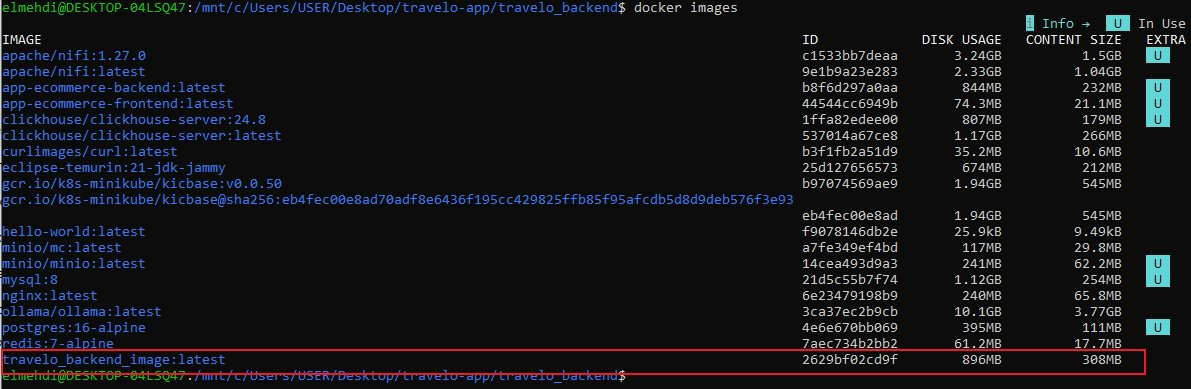
\includegraphics[width=0.95\textwidth]{./screenshots/volet1/08_docker_images_travelo_backend_image_896MB.png}
    \caption{\texttt{docker images} : travelo\_backend\_image:latest (896MB)}
\end{figure}

\subsubsection{5.b. Scan des vulnérabilités}

\begin{lstlisting}[language=bash]
trivy image --timeout 30m travelo_backend_image
\end{lstlisting}

405 vulnérabilités OS (Ubuntu 24.04) + 35 dans le JAR. Recommandation : utiliser \texttt{eclipse-temurin:23-jre-alpine} pour réduire la surface d'attaque.

\begin{figure}[H]
    \centering
    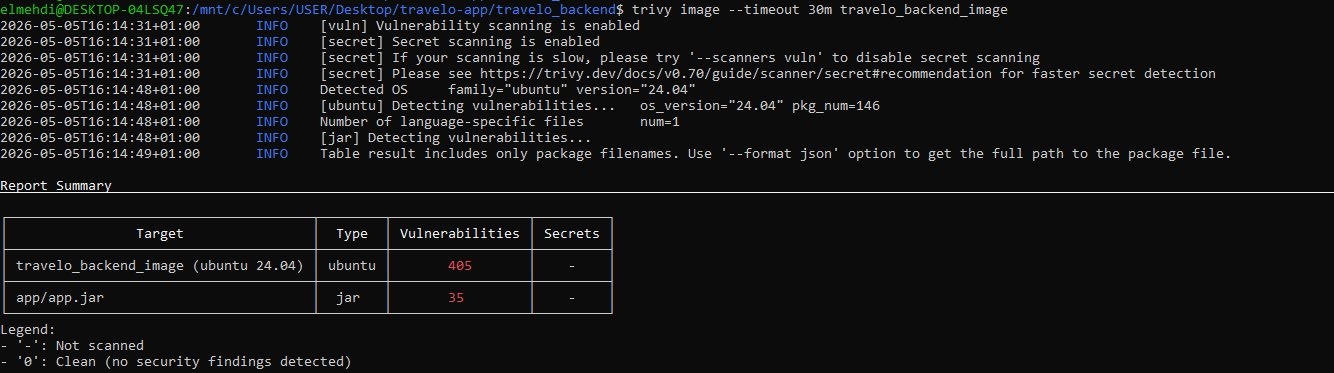
\includegraphics[width=0.95\textwidth]{./screenshots/volet1/09_trivy_scan_backend_405_vulnerabilites_OS_35_JAR.png}
    \caption{Trivy : 405 vulnérabilités OS + 35 JAR sur travelo\_backend\_image}
\end{figure}

\subsubsection{5.c. Publication sur Docker Hub}

\begin{lstlisting}[language=bash]
docker login -u elmehdift37
docker tag travelo_backend_image elmehdift37/travelo-backend:1.0
docker push elmehdift37/travelo-backend:1.0
\end{lstlisting}

\begin{figure}[H]
    \centering
    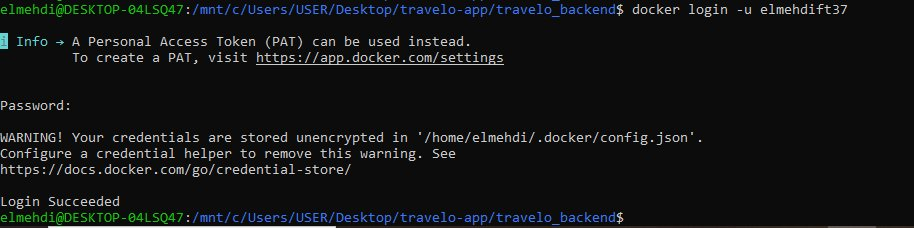
\includegraphics[width=0.95\textwidth]{./screenshots/volet1/10_connexion_docker_hub_reussie.png}
    \caption{Connexion Docker Hub réussie}
\end{figure}

\begin{figure}[H]
    \centering
    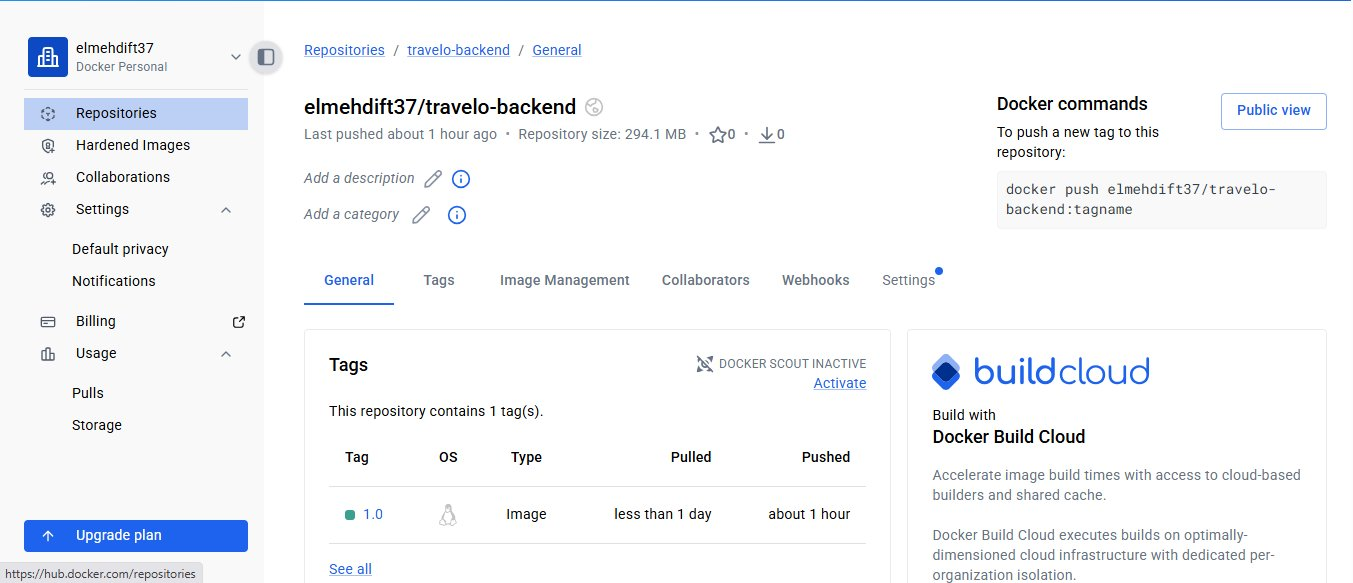
\includegraphics[width=0.95\textwidth]{./screenshots/volet1/11_push_travelo_backend_1.0_docker_hub.png}
    \caption{elmehdift37/travelo-backend:1.0 publié sur Docker Hub}
\end{figure}

\subsubsection{5.d. Lancement du conteneur Backend}

\begin{lstlisting}[language=bash]
docker run -d --name travelo-backend --network travelo-network -p 8080:8080 \
  -e SPRING_DATASOURCE_URL=jdbc:mysql://travelo_app:3306/travelo_db \
  -e SPRING_DATASOURCE_USERNAME=root -e SPRING_DATASOURCE_PASSWORD=password \
  elmehdift37/travelo-backend:1.0
\end{lstlisting}

\begin{figure}[H]
    \centering
    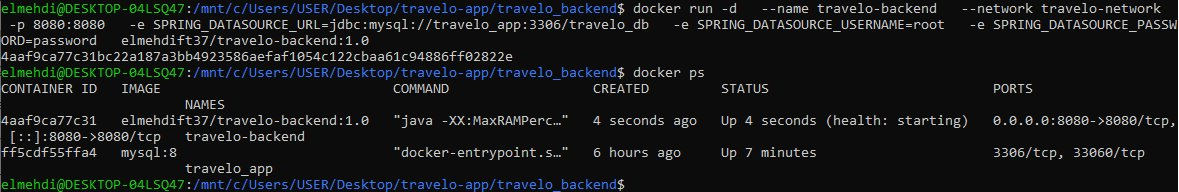
\includegraphics[width=0.95\textwidth]{./screenshots/volet1/12_conteneur_backend_demarre_docker_ps.png}
    \caption{Conteneur travelo-backend démarré (docker ps)}
\end{figure}

\begin{figure}[H]
    \centering
    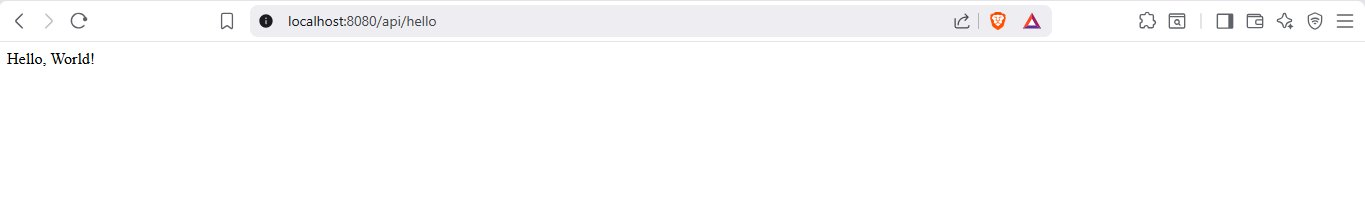
\includegraphics[width=0.95\textwidth]{./screenshots/volet1/13_api_backend_hello_world_localhost_8080.png}
    \caption{API Backend opérationnelle : "Hello, World!" sur localhost:8080/api/hello}
\end{figure}

\subsubsection{5.e. Inspection du conteneur Backend}

\begin{lstlisting}[language=bash]
docker inspect travelo-backend
\end{lstlisting}

\begin{figure}[H]
    \centering
    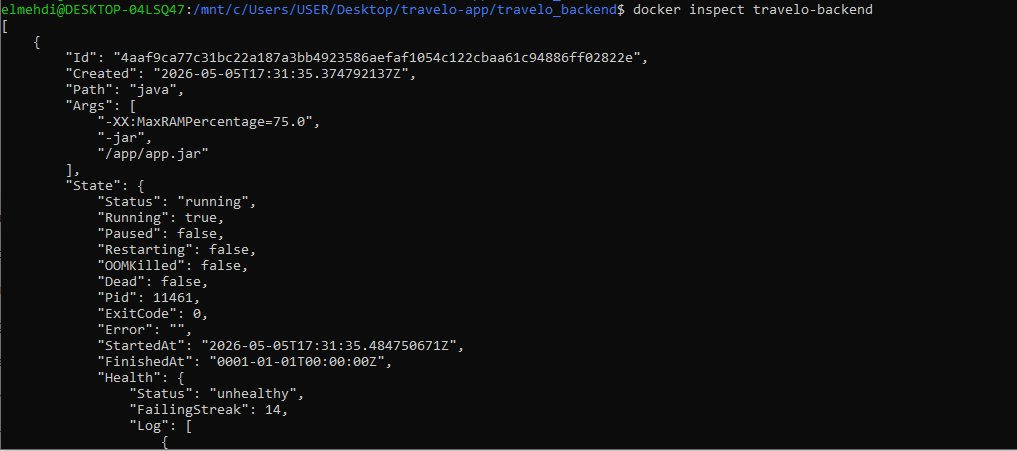
\includegraphics[width=0.95\textwidth]{./screenshots/volet1/14_docker_inspect_backend_running_healthcheck.png}
    \caption{\texttt{docker inspect travelo-backend} : état running, healthcheck configuré}
\end{figure}

\subsubsection{5.f. Logs du conteneur Backend}

\begin{lstlisting}[language=bash]
docker logs travelo-backend
\end{lstlisting}

\begin{figure}[H]
    \centering
    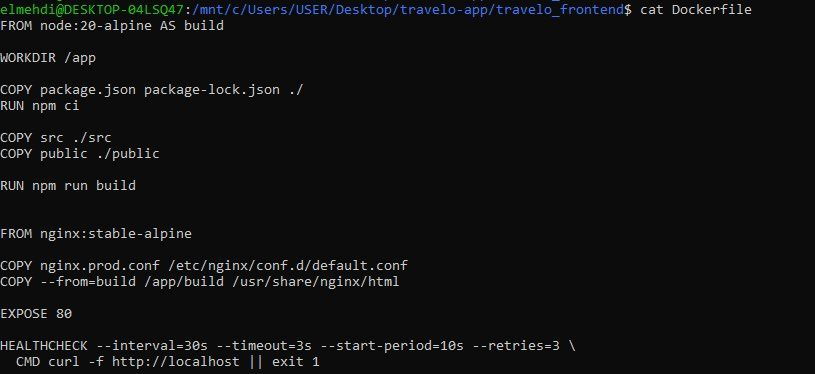
\includegraphics[width=0.95\textwidth]{./screenshots/volet1/15_logs_backend_spring_boot_v3.4.0_port_8080.png}
    \caption{Logs travelo-backend : Spring Boot v3.4.0 démarré sur port 8080}
\end{figure}



\subsection{6. Dockerfile Frontend \& Image}

\begin{figure}[H]
    \centering
    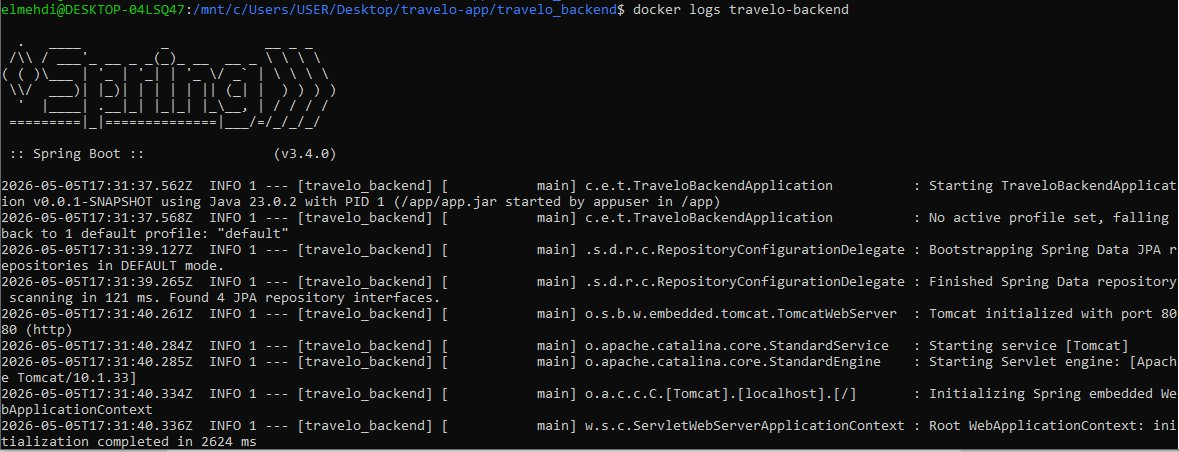
\includegraphics[width=0.95\textwidth]{./screenshots/volet1/16_dockerfile_frontend_node20_alpine_nginx_alpine.png}
    \caption{Dockerfile Frontend : Node:20-alpine (build) + nginx:stable-alpine (runtime)}
\end{figure}

\subsubsection{Bonnes pratiques Frontend}

\begin{itemize}
    \item Multi-stage build Node → Nginx Alpine (\textasciitilde{}95MB)
    \item \texttt{npm ci} pour builds reproductibles
    \item \texttt{package.json} copié séparément pour le cache
    \item HEALTHCHECK Nginx
    \item EXPOSE 80
\end{itemize}

\begin{lstlisting}[language=bash]
docker build -t travelo-frontend .
\end{lstlisting}

\begin{figure}[H]
    \centering
    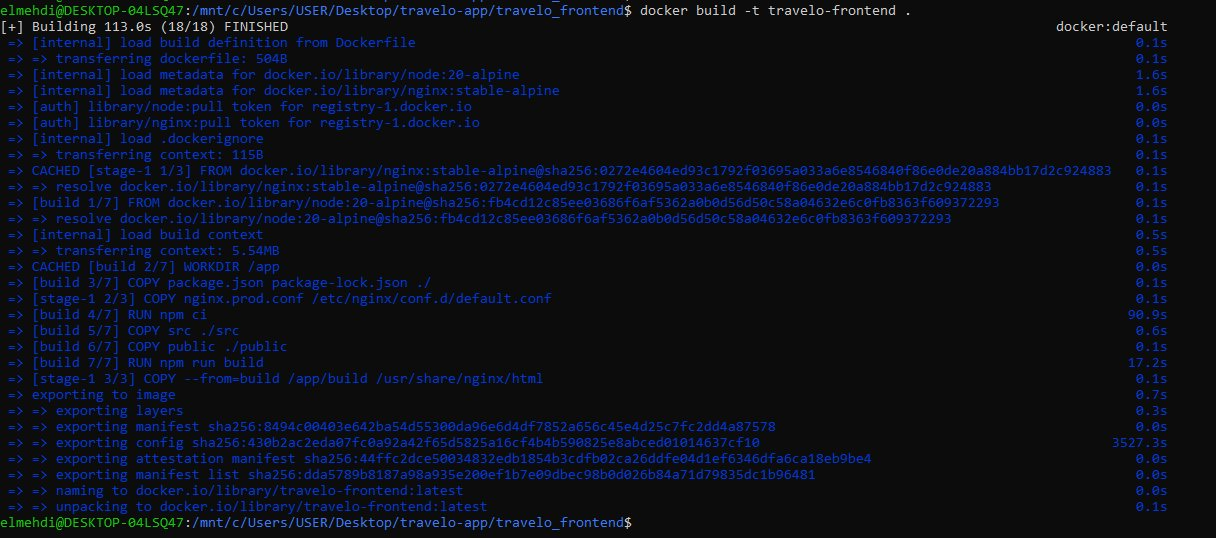
\includegraphics[width=0.95\textwidth]{./screenshots/volet1/17_build_frontend_travelo_succes_18_etapes_95MB.png}
    \caption{Build travelo-frontend réussi (18/18 étapes, 95.2MB)}
\end{figure}

\begin{figure}[H]
    \centering
    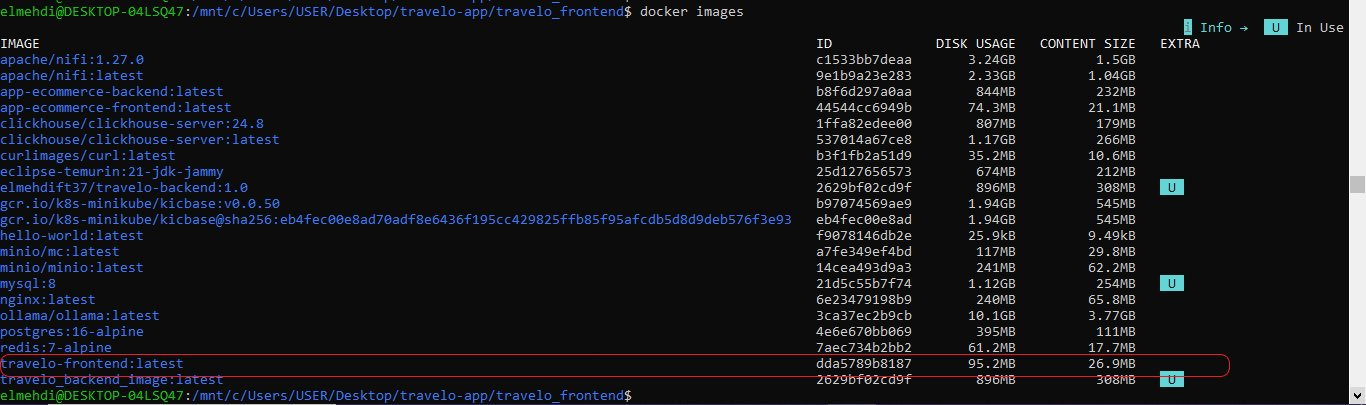
\includegraphics[width=0.95\textwidth]{./screenshots/volet1/18_docker_images_travelo_frontend_et_backend.png}
    \caption{\texttt{docker images} : travelo-frontend:latest et travelo\_backend\_image:latest}
\end{figure}

\subsubsection{Scan Trivy Frontend}

\begin{lstlisting}[language=bash]
trivy image travelo-frontend
\end{lstlisting}

3 vulnérabilités (2 MEDIUM, 1 HIGH) sur Alpine 3.23.4 : libxpm, nghttp2-libs, xz-libs. Toutes disposent de versions corrigées disponibles via mise à jour de l'image de base.

\begin{figure}[H]
    \centering
    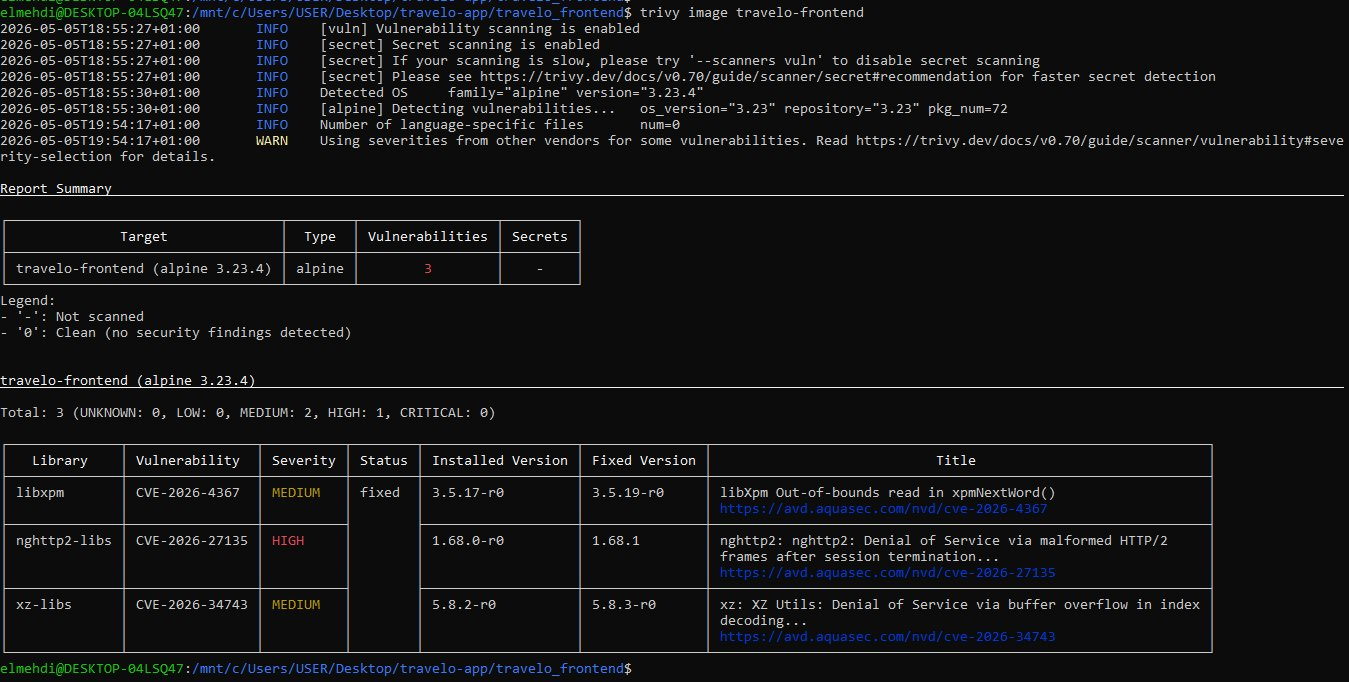
\includegraphics[width=0.95\textwidth]{./screenshots/volet1/19_trivy_scan_frontend_3_vulnerabilites_alpine.png}
    \caption{Trivy frontend : 3 vulnérabilités (libxpm, nghttp2-libs, xz-libs)}
\end{figure}

\subsubsection{Publication Frontend sur Docker Hub}

\begin{lstlisting}[language=bash]
docker tag travelo-frontend elmehdift37/travelo-frontend:1.0
docker push elmehdift37/travelo-frontend:1.0
\end{lstlisting}

\begin{figure}[H]
    \centering
    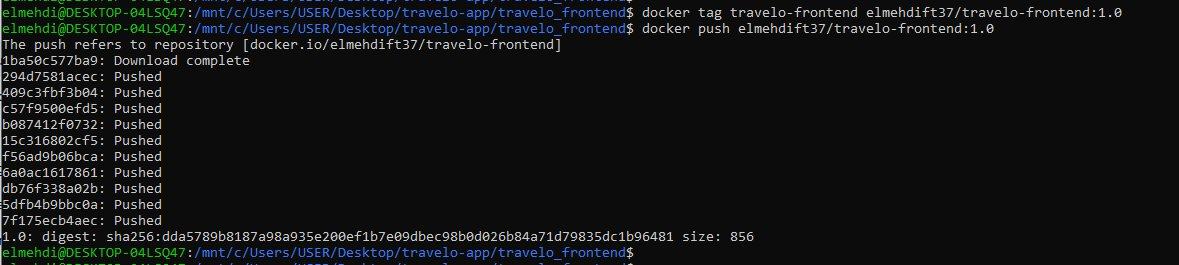
\includegraphics[width=0.95\textwidth]{./screenshots/volet1/20_push_travelo_frontend_1.0_docker_hub.png}
    \caption{Push travelo-frontend:1.0 vers Docker Hub}
\end{figure}

\begin{figure}[H]
    \centering
    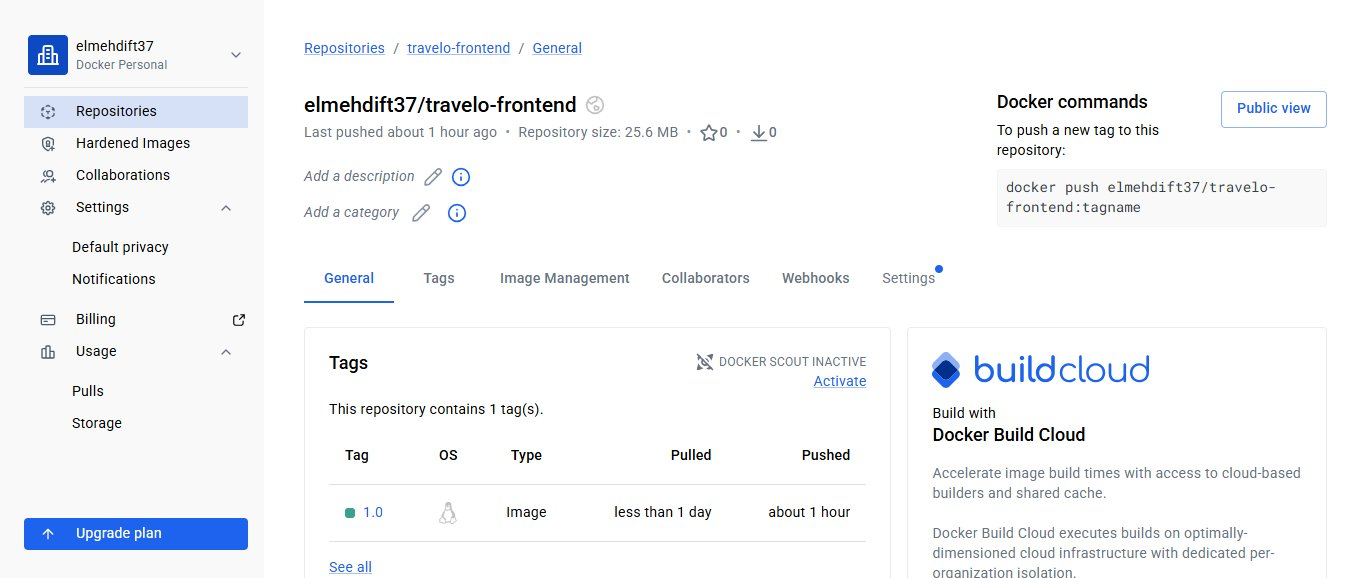
\includegraphics[width=0.95\textwidth]{./screenshots/volet1/21_docker_hub_travelo_frontend_tag_1.0_25MB.png}
    \caption{elmehdift37/travelo-frontend sur Docker Hub (tag 1.0, 25.6MB)}
\end{figure}

\subsubsection{Lancement du conteneur Frontend}

\begin{lstlisting}[language=bash]
docker run -d --name travelo-frontend --network travelo-network -p 3000:80 elmehdift37/travelo-frontend:1.0
\end{lstlisting}

\begin{figure}[H]
    \centering
    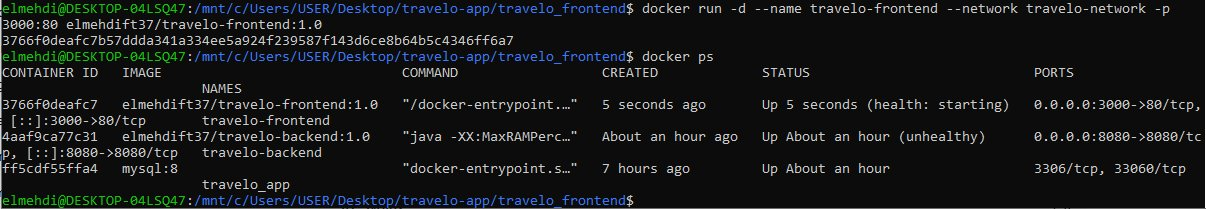
\includegraphics[width=0.95\textwidth]{./screenshots/volet1/22_docker_ps_3_conteneurs_mysql_backend_frontend_actifs.png}
    \caption{Les 3 conteneurs actifs : mysql, travelo-backend, travelo-frontend}
\end{figure}



\subsection{7. Vérification du bon fonctionnement de l'application}

Les trois conteneurs étant démarrés, l'application Travelo est accessible depuis le navigateur sur localhost:3000.

\begin{figure}[H]
    \centering
    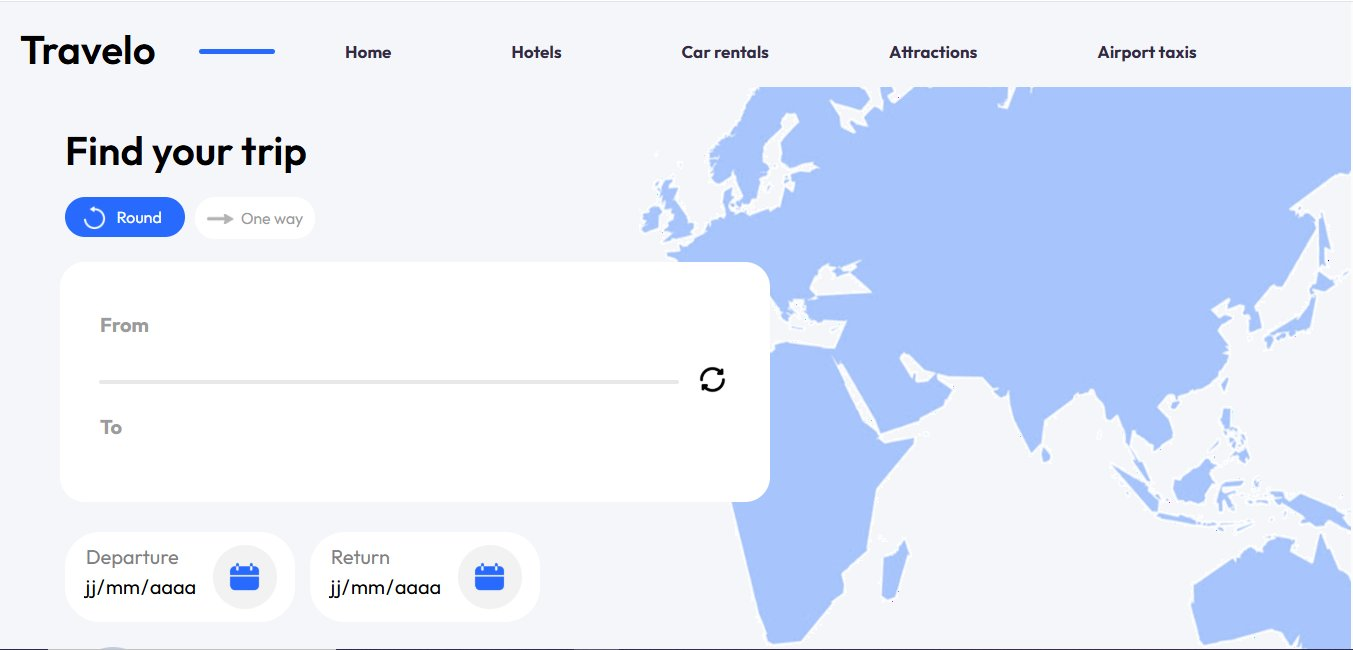
\includegraphics[width=0.95\textwidth]{./screenshots/volet1/23_interface_travelo_localhost_3000_find_your_trip.png}
    \caption{Interface Travelo sur localhost:3000 : page "Find your trip"}
\end{figure}

\subsubsection{Inspection du Frontend}

\begin{lstlisting}[language=bash]
docker inspect travelo-frontend
\end{lstlisting}

\begin{figure}[H]
    \centering
    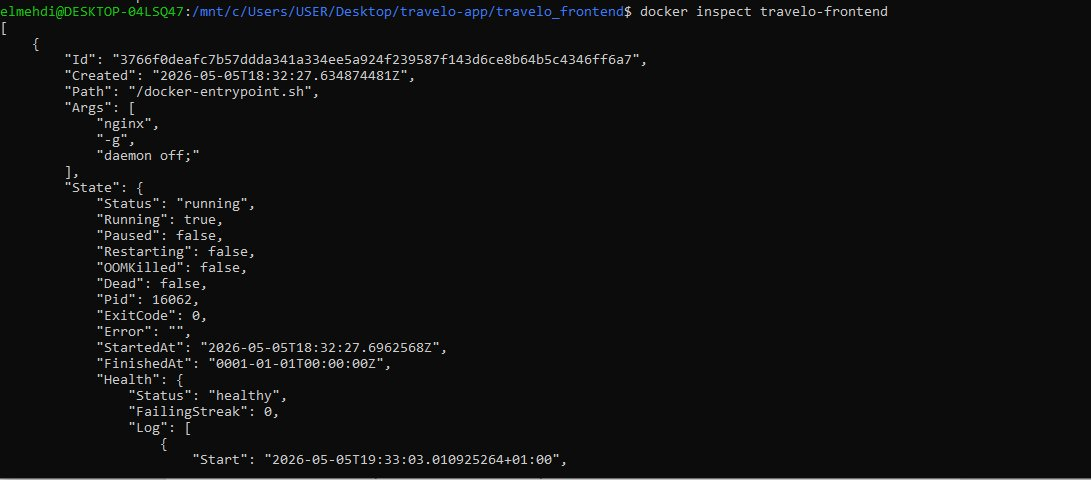
\includegraphics[width=0.95\textwidth]{./screenshots/volet1/24_docker_inspect_frontend_running_healthy.png}
    \caption{\texttt{docker inspect travelo-frontend} : état running, health: healthy}
\end{figure}

\subsubsection{Logs du Frontend}

\begin{lstlisting}[language=bash]
docker logs travelo-frontend
\end{lstlisting}

\begin{figure}[H]
    \centering
    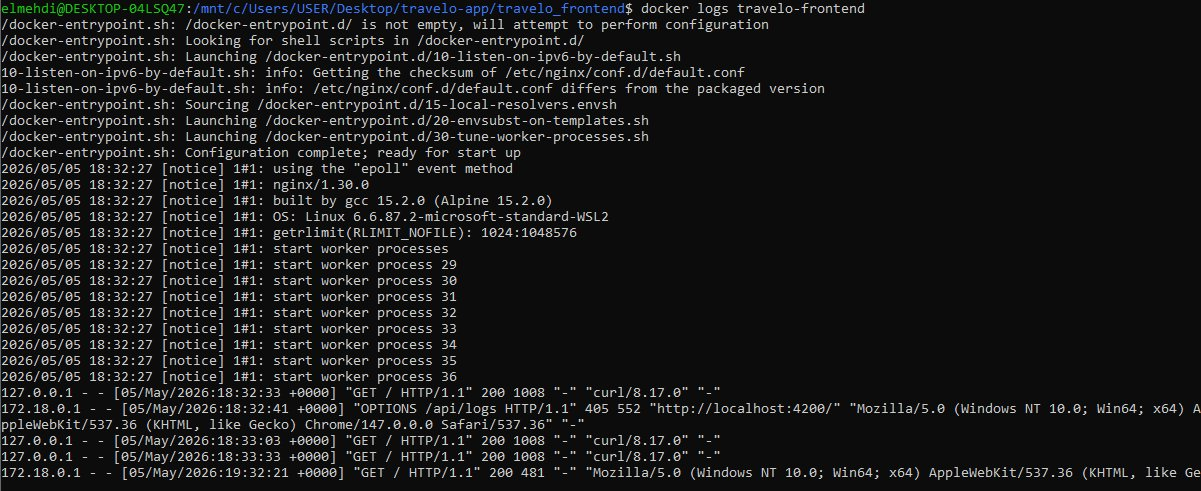
\includegraphics[width=0.95\textwidth]{./screenshots/volet1/25_logs_nginx_1.30.0_demarrage_requetes_http.png}
    \caption{Logs Nginx 1.30.0 : démarrage et requêtes HTTP traitées}
\end{figure}

\subsubsection{Test fonctionnel – Formulaire de réservation}

\begin{figure}[H]
    \centering
    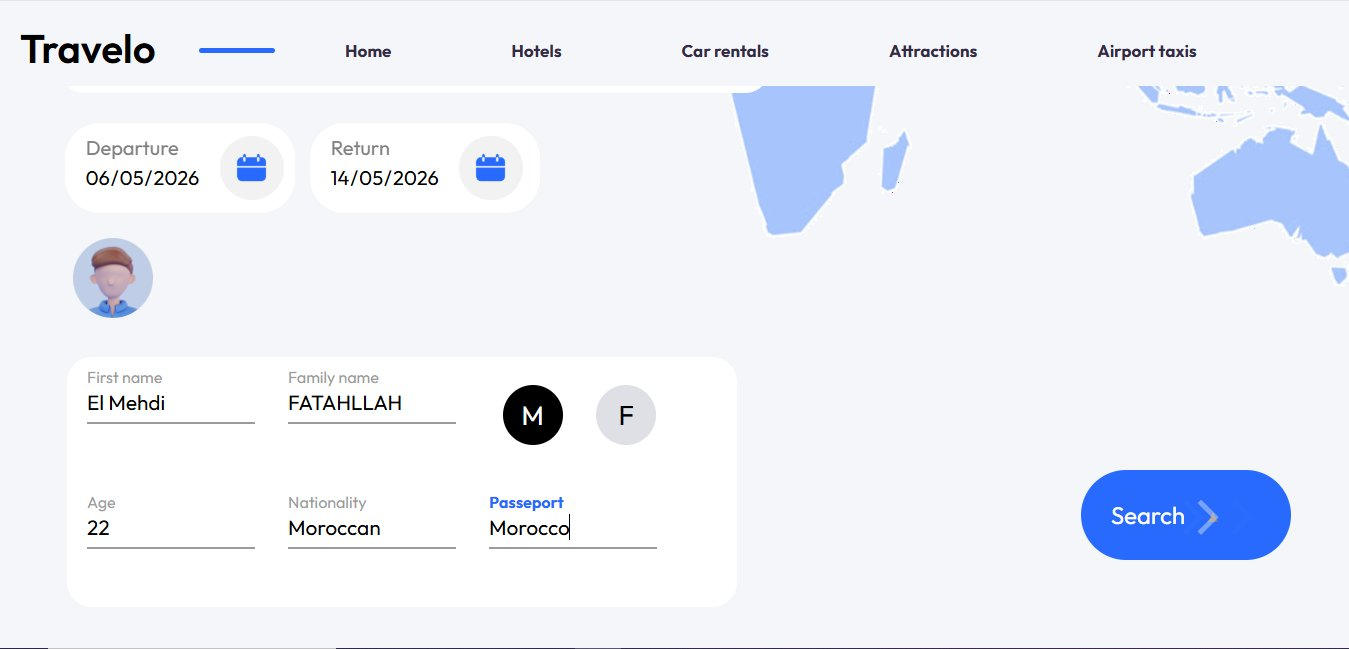
\includegraphics[width=0.95\textwidth]{./screenshots/volet1/26_formulaire_passager_elmehdi_fatahllah_moroccan.png}
    \caption{Formulaire passager renseigné (El Mehdi FATAHLLAH, Moroccan)}
\end{figure}



\subsection{8. Suppression des conteneurs}

\begin{lstlisting}[language=bash]
docker rm -f travelo-backend travelo-frontend travelo_app
\end{lstlisting}

\begin{itemize}
    \item \texttt{docker rm -f} : Suppression forcée des conteneurs, même en cours d'exécution
\end{itemize}

\begin{figure}[H]
    \centering
    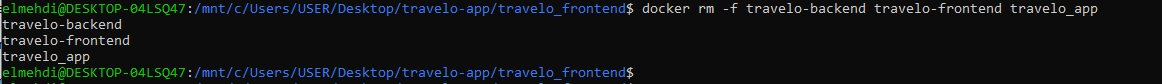
\includegraphics[width=0.95\textwidth]{./screenshots/volet1/27_suppression_forcee_3_conteneurs_docker_rm.png}
    \caption{Suppression forcée des 3 conteneurs}
\end{figure}

\begin{figure}[H]
    \centering
    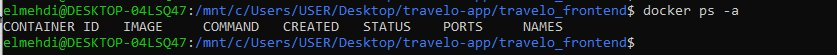
\includegraphics[width=0.95\textwidth]{./screenshots/volet1/28_docker_ps_aucun_conteneur_restant.png}
    \caption{\texttt{docker ps -a} : aucun conteneur actif restant}
\end{figure}



\subsection{9. Redéploiement avec Docker Compose}

\subsubsection{9.a. Fichier docker-compose.yml}

\begin{figure}[H]
    \centering
    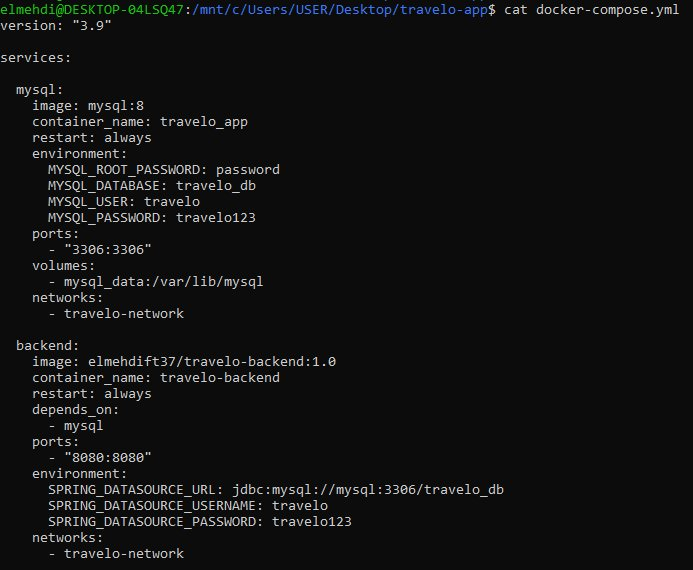
\includegraphics[width=0.95\textwidth]{./screenshots/volet1/29_docker_compose_yml_services_mysql_backend.png}
    \caption{docker-compose.yml : services mysql et backend}
\end{figure}

\begin{figure}[H]
    \centering
    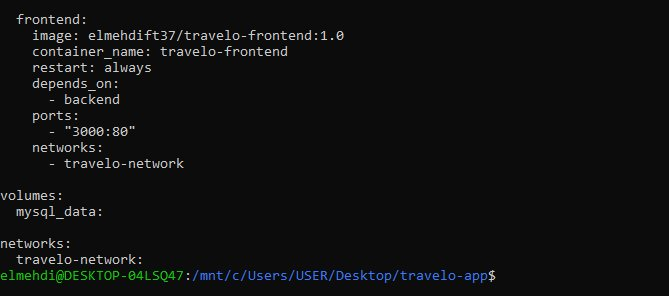
\includegraphics[width=0.95\textwidth]{./screenshots/volet1/30_docker_compose_yml_service_frontend_volumes_reseau.png}
    \caption{docker-compose.yml : service frontend, volumes et réseau}
\end{figure}

Points clés : \texttt{depends\_on} (ordre de démarrage), \texttt{restart: always}, réseau commun \texttt{travelo-network}, volume \texttt{mysql\_data} persistant.

\subsubsection{9.b. Lancement}

\begin{lstlisting}[language=bash]
docker compose up -d
\end{lstlisting}

\begin{figure}[H]
    \centering
    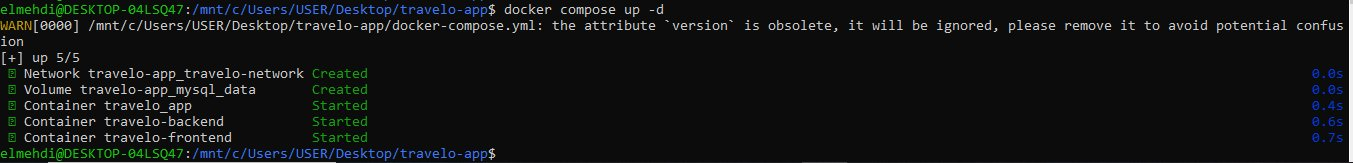
\includegraphics[width=0.95\textwidth]{./screenshots/volet1/31_docker_compose_up_reseau_volume_3_conteneurs_crees.png}
    \caption{docker compose up -d : réseau, volume et 3 conteneurs créés}
\end{figure}

\begin{figure}[H]
    \centering
    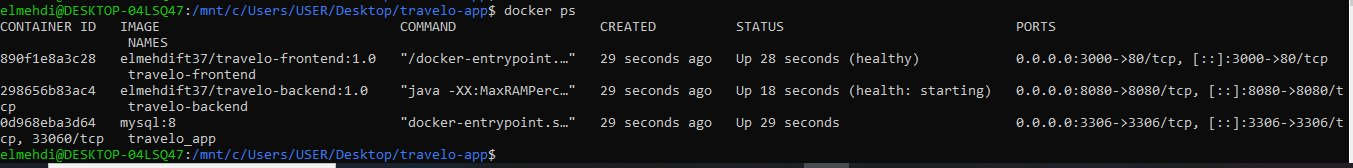
\includegraphics[width=0.95\textwidth]{./screenshots/volet1/32_docker_ps_3_conteneurs_up_avec_ports.png}
    \caption{\texttt{docker ps} : les 3 conteneurs "Up" avec leurs ports}
\end{figure}

\subsubsection{9.c. Vérification}

\begin{figure}[H]
    \centering
    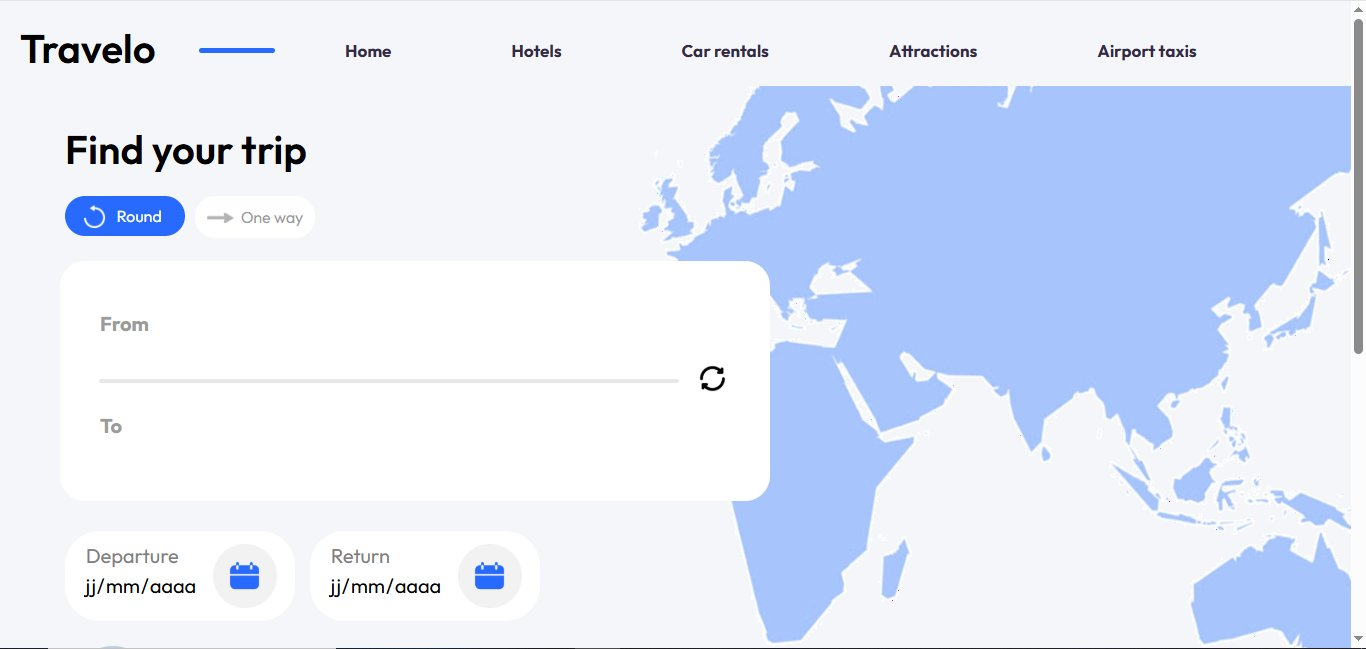
\includegraphics[width=0.95\textwidth]{./screenshots/volet1/33_travelo_fonctionnel_docker_compose_localhost_3000.png}
    \caption{Application Travelo fonctionnelle via Docker Compose (localhost:3000)}
\end{figure}



\subsection{10. Suppression des conteneurs et images}

\begin{lstlisting}[language=bash]
docker rm -f travelo-backend travelo-frontend travelo_app
docker rmi -f elmehdift37/travelo-frontend:1.0 elmehdift37/travelo-backend:1.0 mysql:8
\end{lstlisting}

\begin{figure}[H]
    \centering
    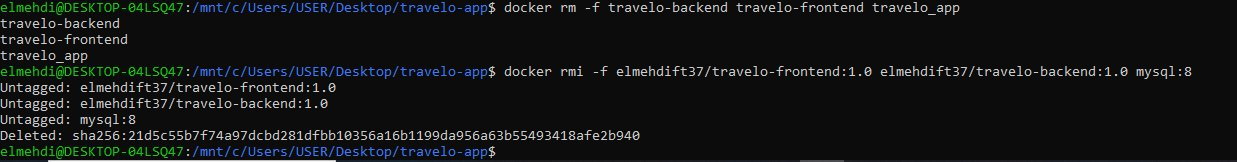
\includegraphics[width=0.95\textwidth]{./screenshots/volet1/34_suppression_conteneurs_et_images_docker_locales.png}
    \caption{Suppression des conteneurs et des images Docker locales}
\end{figure}



\subsection{11. Registre privé local d'images Docker}

Un registre privé Docker est déployé localement via deux services : \texttt{registry:2} (port 5000) pour le stockage, et \texttt{joxit/docker-registry-ui} (port 8081) pour la visualisation via navigateur.

\subsubsection{Fichier docker-compose.yml du registre}

\begin{figure}[H]
    \centering
    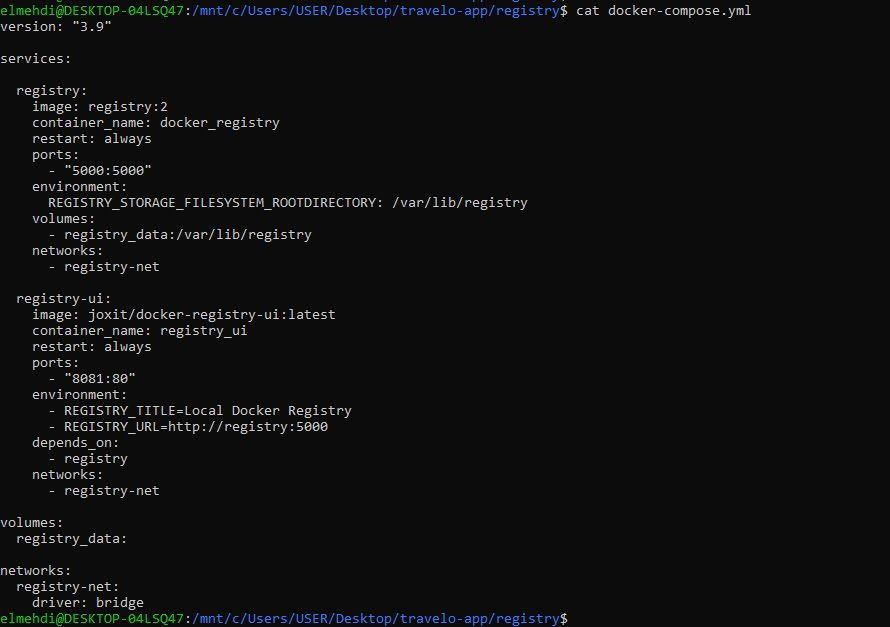
\includegraphics[width=0.95\textwidth]{./screenshots/volet1/35_docker_compose_yml_registre_prive_registry2_ui.png}
    \caption{docker-compose.yml du registre privé (registry:2 + docker-registry-ui)}
\end{figure}

\subsubsection{Démarrage du registre}

\begin{lstlisting}[language=bash]
docker compose up -d
\end{lstlisting}

\begin{figure}[H]
    \centering
    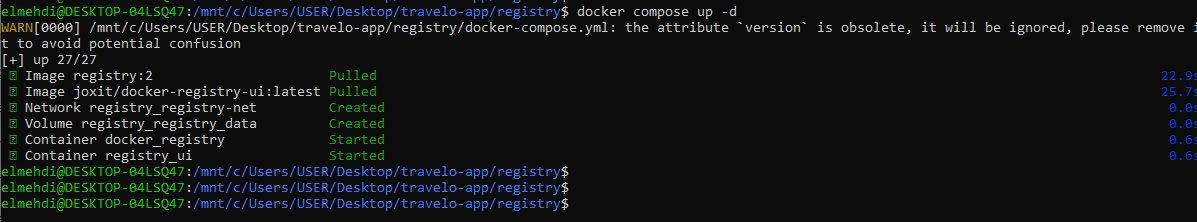
\includegraphics[width=0.95\textwidth]{./screenshots/volet1/36_demarrage_registre_docker_registry_port5000_ui_port8081.png}
    \caption{Démarrage du registre : docker\_registry (port 5000) et registry\_ui (port 8081)}
\end{figure}

\begin{figure}[H]
    \centering
    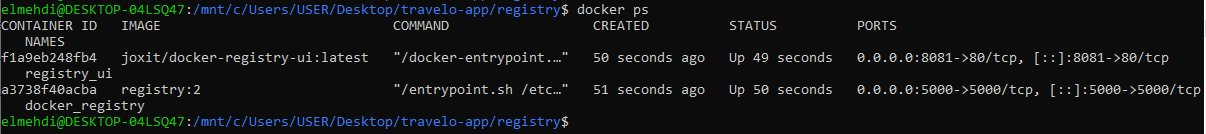
\includegraphics[width=0.95\textwidth]{./screenshots/volet1/37_docker_ps_registry2_et_registry_ui_actifs.png}
    \caption{\texttt{docker ps} : registry:2 et registry\_ui actifs}
\end{figure}

\subsubsection{Push des images vers le registre privé}

\begin{lstlisting}[language=bash]
docker tag travelo-frontend localhost:5000/travelo-frontend:1.0
docker push localhost:5000/travelo-frontend:1.0
docker tag elmehdift37/travelo-backend:1.0 localhost:5000/travelo-backend:1.0
docker push localhost:5000/travelo-backend:1.0
\end{lstlisting}

\begin{figure}[H]
    \centering
    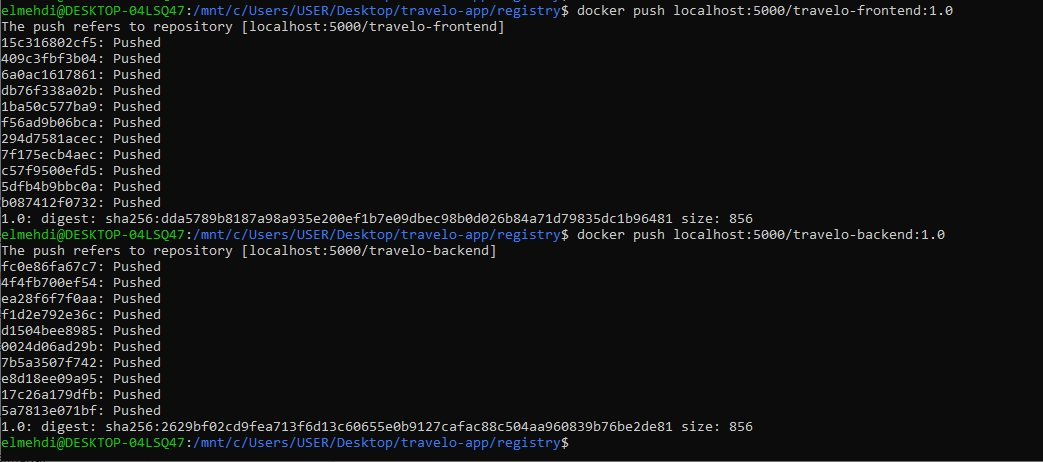
\includegraphics[width=0.95\textwidth]{./screenshots/volet1/38_push_images_vers_localhost_5000_backend_frontend.png}
    \caption{Push des deux images vers localhost:5000}
\end{figure}

\subsubsection{Visualisation via l'interface UI}

\begin{figure}[H]
    \centering
    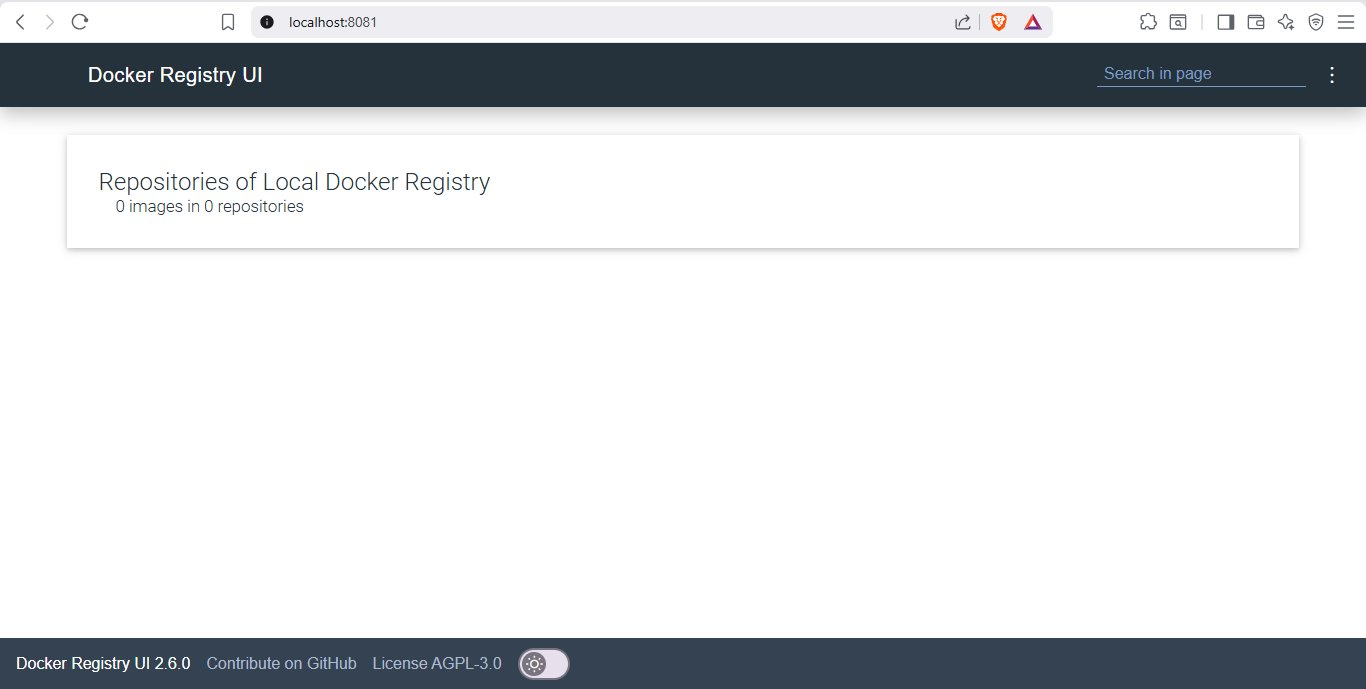
\includegraphics[width=0.95\textwidth]{./screenshots/volet1/39_docker_registry_ui_vide_localhost_8081.png}
    \caption{Docker Registry UI vide au démarrage (localhost:8081)}
\end{figure}

\begin{figure}[H]
    \centering
    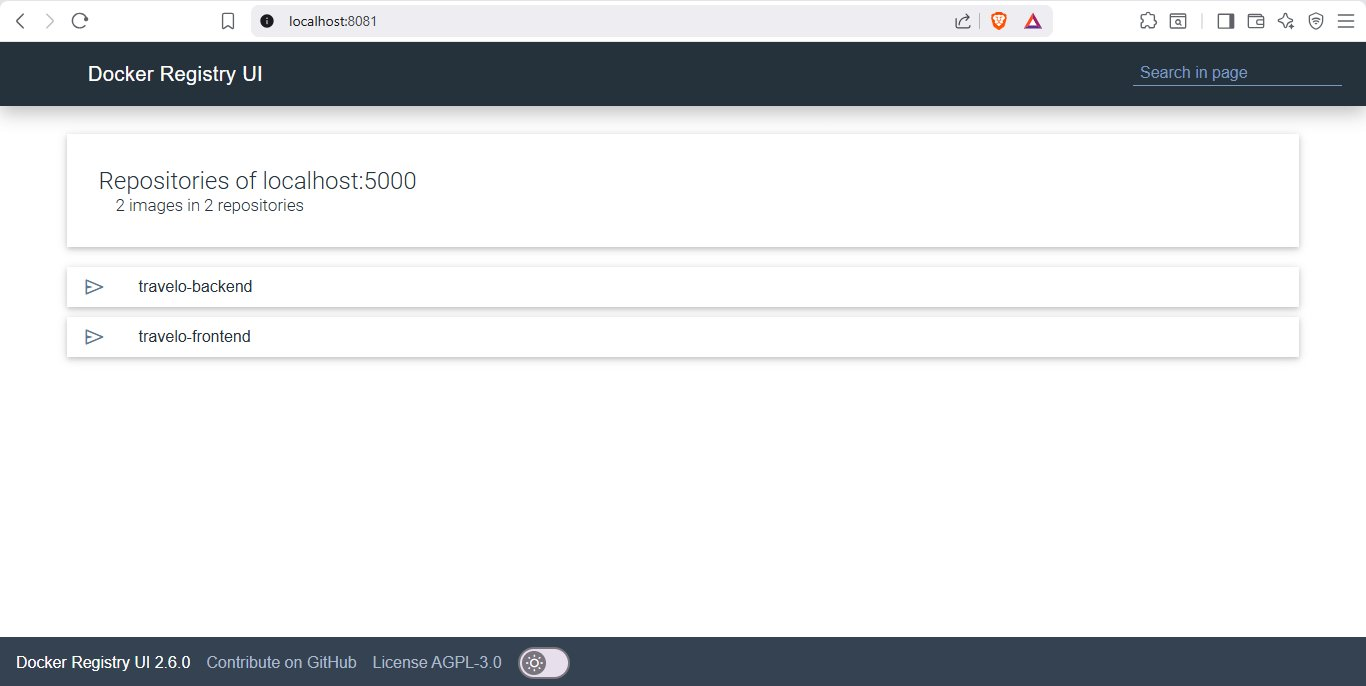
\includegraphics[width=0.95\textwidth]{./screenshots/volet1/40_docker_registry_ui_2_depots_backend_frontend.png}
    \caption{Docker Registry UI : 2 images dans 2 dépôts (travelo-backend, travelo-frontend)}
\end{figure}

\begin{figure}[H]
    \centering
    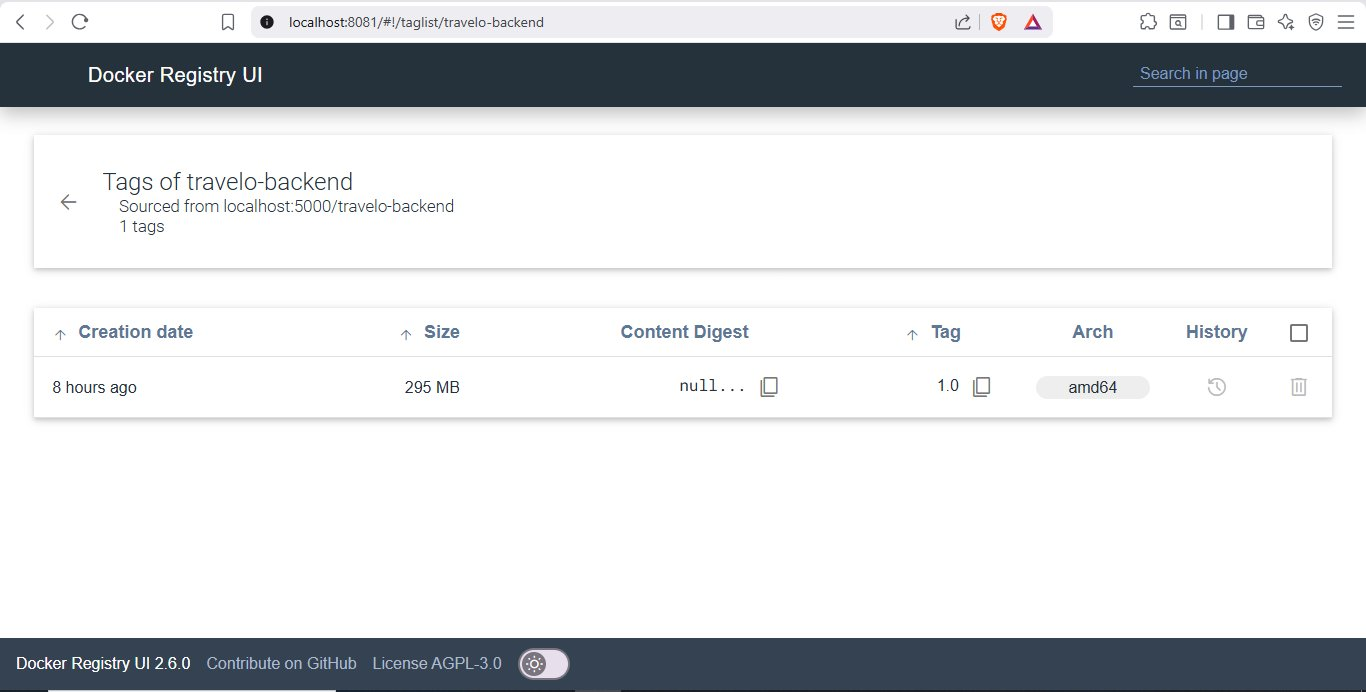
\includegraphics[width=0.95\textwidth]{./screenshots/volet1/41_detail_depot_travelo_backend_tag1.0_295MB_amd64.png}
    \caption{Détail du dépôt travelo-backend : tag 1.0, 295MB, architecture amd64}
\end{figure}

\begin{figure}[H]
    \centering
    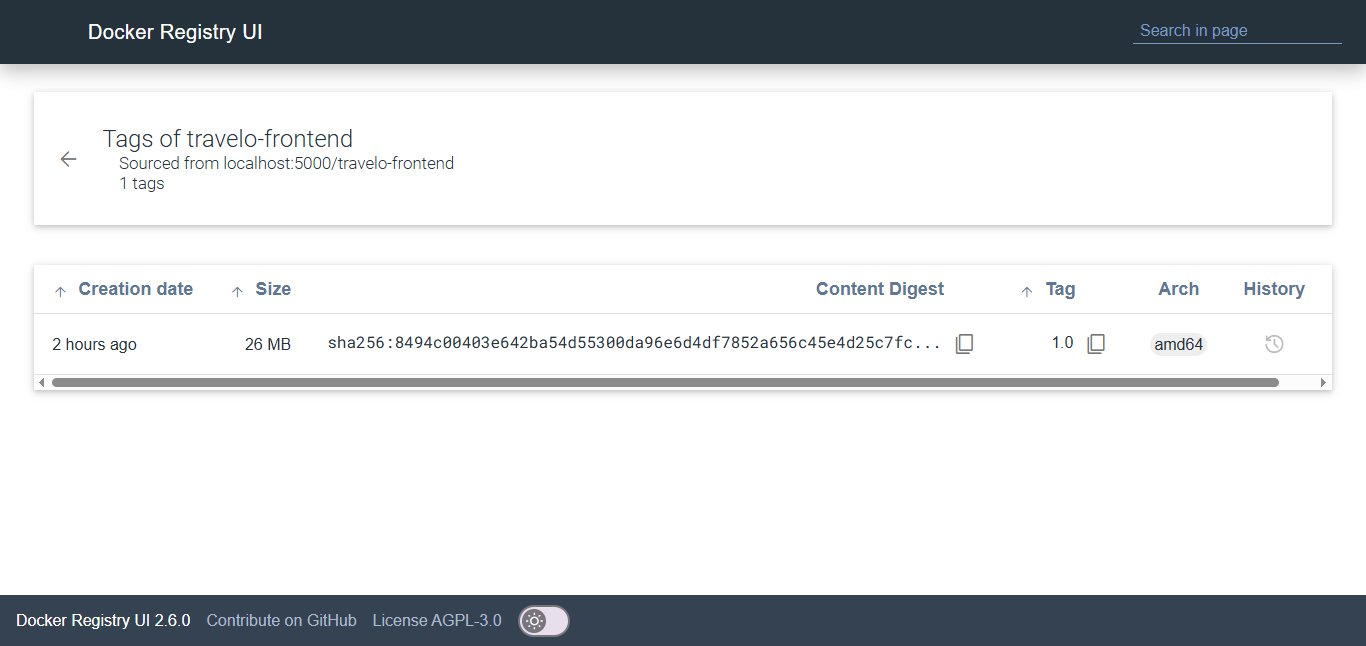
\includegraphics[width=0.95\textwidth]{./screenshots/volet1/42_detail_depot_travelo_frontend_tag1.0_digest_sha256.png}
    \caption{Détail du dépôt travelo-frontend : tag 1.0, digest SHA256 visible}
\end{figure}



\subsection{12. Redéploiement depuis le registre privé}

Un nouveau fichier docker-compose.yml est créé en remplaçant les références Docker Hub par \texttt{localhost:5000} pour utiliser les images du registre privé local.

\subsubsection{Fichier docker-compose.yml avec registre privé}

\begin{figure}[H]
    \centering
    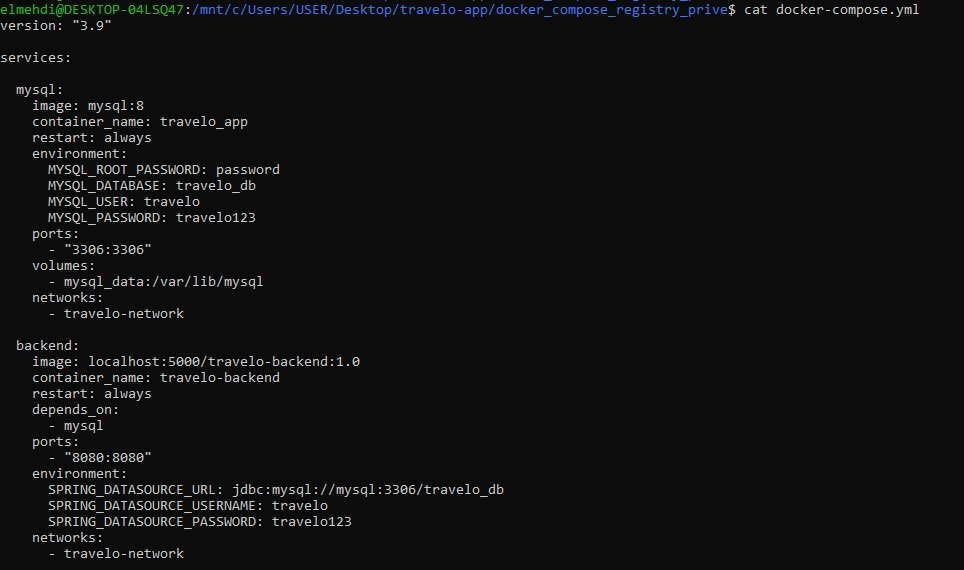
\includegraphics[width=0.95\textwidth]{./screenshots/volet1/43_docker_compose_yml_images_registre_prive_localhost_5000.png}
    \caption{docker-compose.yml avec image: localhost:5000/travelo-backend:1.0 et localhost:5000/travelo-frontend:1.0}
\end{figure}

\begin{figure}[H]
    \centering
    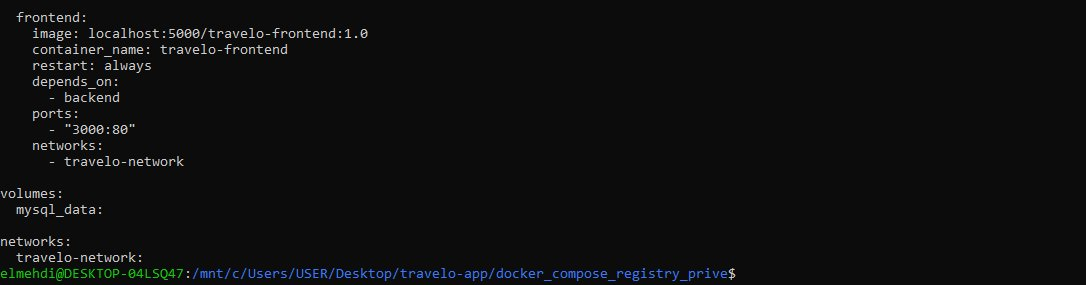
\includegraphics[width=0.95\textwidth]{./screenshots/volet1/44_docker_compose_yml_service_frontend_registre_local_port3000.png}
    \caption{Suite du docker-compose.yml : service frontend depuis le registre local (port 3000)}
\end{figure}

\subsubsection{Démarrage depuis le registre privé}

\begin{lstlisting}[language=bash]
docker compose up -d
\end{lstlisting}

\begin{figure}[H]
    \centering
    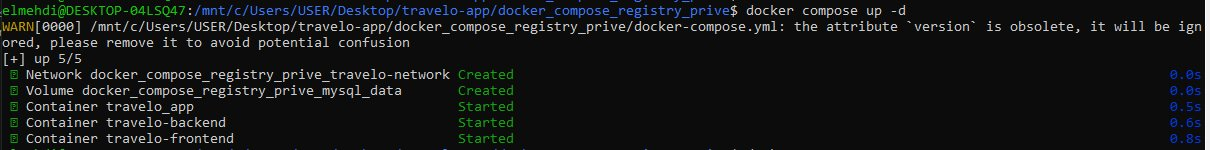
\includegraphics[width=0.95\textwidth]{./screenshots/volet1/45_docker_compose_up_3_conteneurs_depuis_localhost_5000.png}
    \caption{docker compose up -d : réseau, volume et 3 conteneurs démarrés depuis localhost:5000}
\end{figure}

\begin{figure}[H]
    \centering
    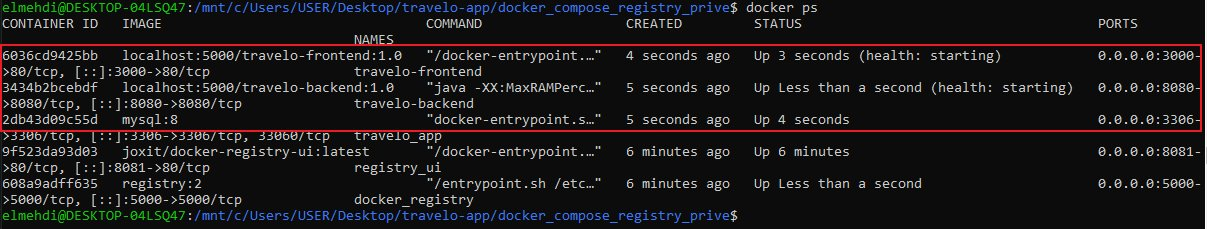
\includegraphics[width=0.95\textwidth]{./screenshots/volet1/46_docker_ps_frontend_backend_depuis_localhost_5000_actifs.png}
    \caption{\texttt{docker ps} : travelo-frontend et travelo-backend tirés depuis localhost:5000, tous actifs}
\end{figure}

\subsubsection{Vérification de l'application}

\begin{figure}[H]
    \centering
    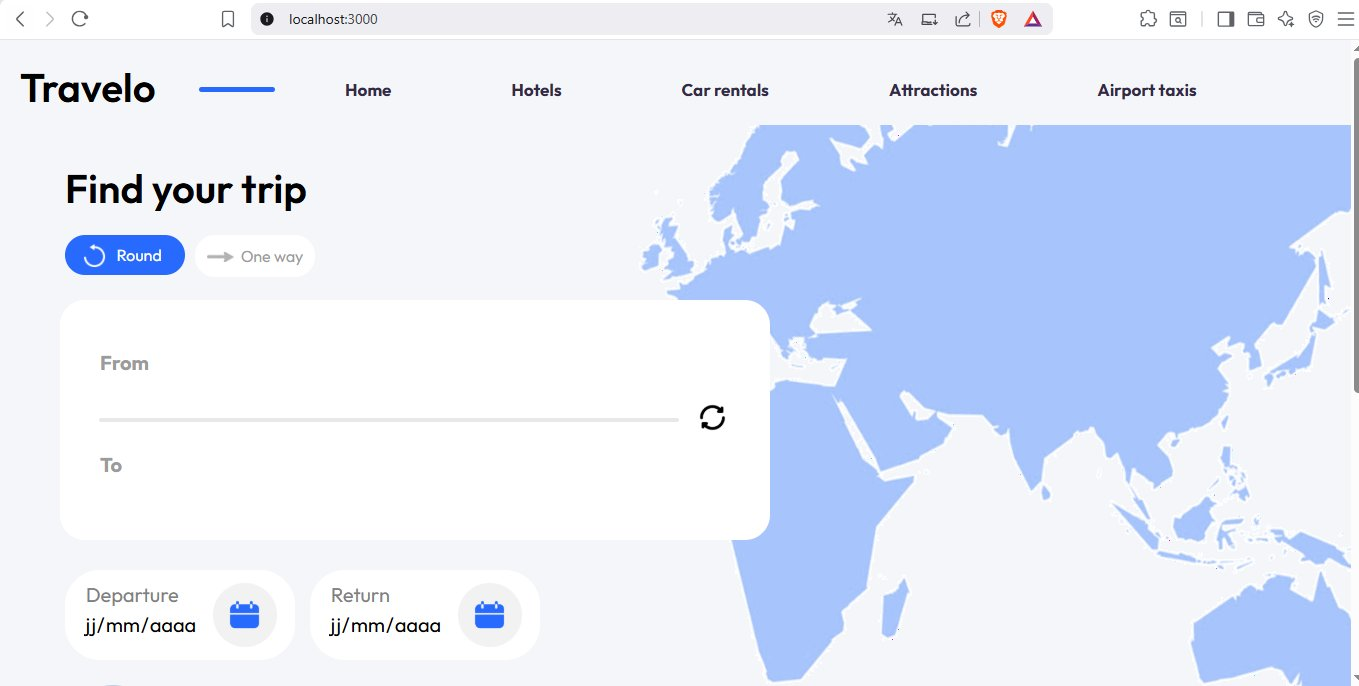
\includegraphics[width=0.95\textwidth]{./screenshots/volet1/47_travelo_fonctionnel_depuis_registre_prive_localhost_3000.png}
    \caption{Application Travelo fonctionnelle depuis le registre privé (localhost:3000)}
\end{figure}



\subsection{Bonus : Déploiement Docker Swarm}

Docker Swarm est un orchestrateur natif de Docker permettant de gérer un cluster de nœuds, d'assurer la haute disponibilité par réplication des services, et d'équilibrer automatiquement la charge.

\subsubsection{Fichier docker-compose.yml compatible Swarm}

Le fichier de stack Swarm définit 4 services : mysql (1 réplica, manager), backend (2 réplicas), frontend (2 réplicas), et traefik (reverse proxy). Chaque service dispose d'une politique de redémarrage et de limites de ressources CPU/mémoire.

\begin{figure}[H]
    \centering
    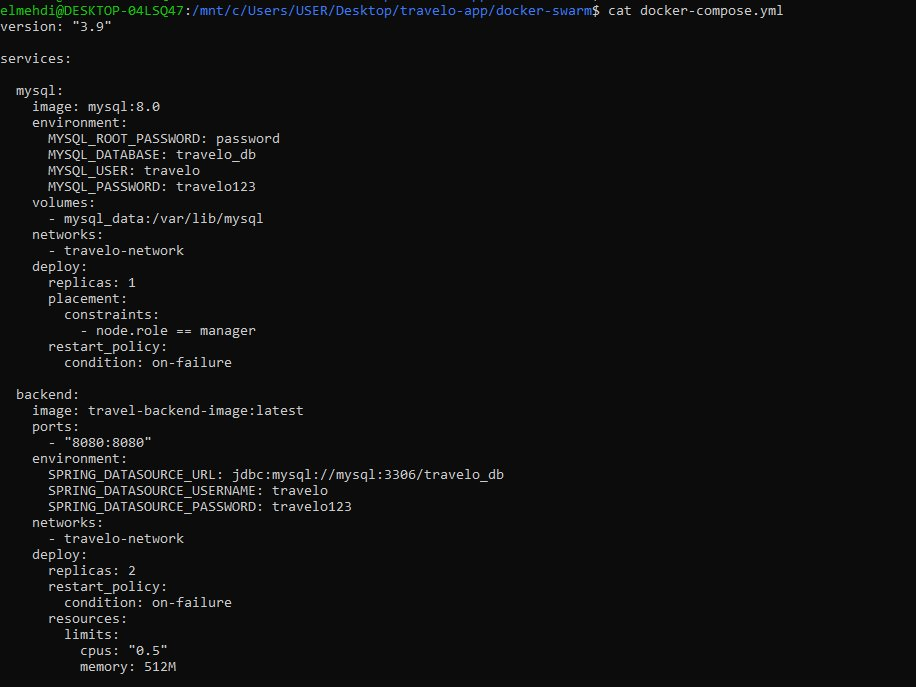
\includegraphics[width=0.95\textwidth]{./screenshots/volet1/48_docker_compose_swarm_services_mysql_backend_replicas.png}
    \caption{docker-compose.yml Swarm : services mysql et backend (réplicas, restart\_policy, resource limits)}
\end{figure}

\begin{figure}[H]
    \centering
    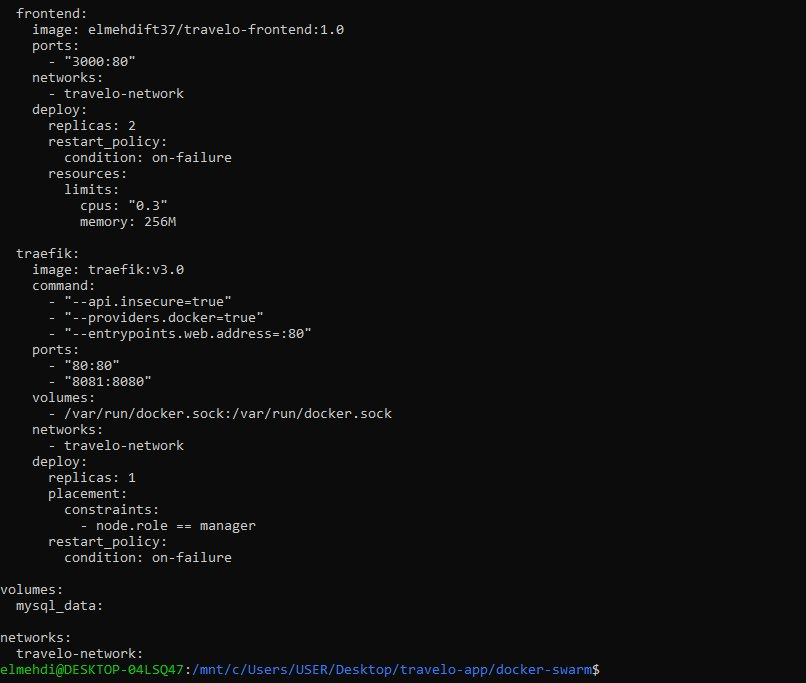
\includegraphics[width=0.95\textwidth]{./screenshots/volet1/49_docker_compose_swarm_service_frontend_2_replicas_traefik.png}
    \caption{docker-compose.yml Swarm : service frontend (2 réplicas, 0.3 CPU, 256M) + Traefik (reverse proxy)}
\end{figure}



\subsection{13. Initialisation du cluster Docker Swarm}

La commande \texttt{docker swarm init} initialise le nœud courant comme manager du cluster. Un token de jonction est généré pour l'ajout de workers.

\begin{lstlisting}[language=bash]
docker swarm init
\end{lstlisting}

\begin{figure}[H]
    \centering
    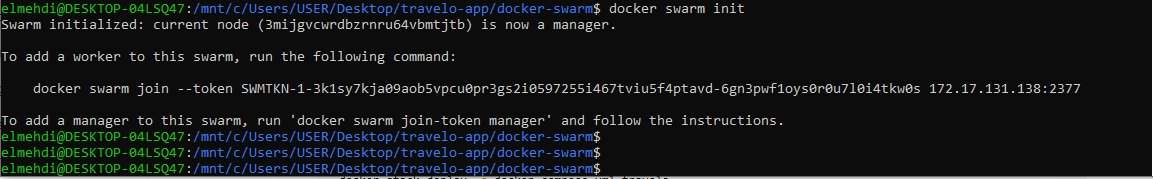
\includegraphics[width=0.95\textwidth]{./screenshots/volet1/50_docker_swarm_init_noeud_manager_leader.png}
    \caption{docker swarm init : nœud DESKTOP-04LSQ47 initialisé comme manager (Leader)}
\end{figure}

\subsubsection{Vérification des nœuds}

\begin{lstlisting}[language=bash]
docker node ls
\end{lstlisting}

\begin{figure}[H]
    \centering
    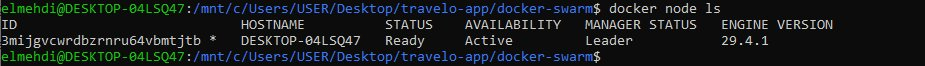
\includegraphics[width=0.95\textwidth]{./screenshots/volet1/51_docker_node_ls_1_noeud_manager_ready_leader.png}
    \caption{\texttt{docker node ls} : 1 nœud manager actif (Status: Ready, Manager Status: Leader)}
\end{figure}



\subsection{14 \& 15. Déploiement de la stack avec réplicas et limites de ressources}

La stack est déployée via \texttt{docker stack deploy} en utilisant le fichier docker-compose.yml. Chaque service est créé avec ses réplicas et ses contraintes de ressources définies dans la section \texttt{deploy}.

\begin{lstlisting}[language=bash]
docker stack deploy -c docker-compose.yml travelo_swarm
\end{lstlisting}

\begin{figure}[H]
    \centering
    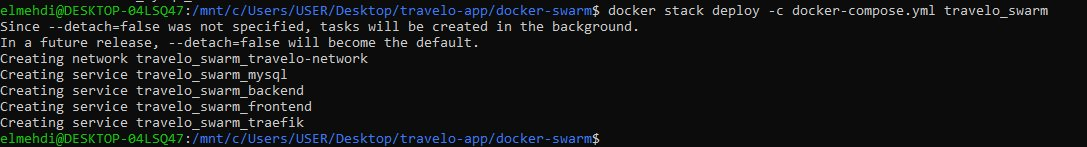
\includegraphics[width=0.95\textwidth]{./screenshots/volet1/52_stack_travelo_swarm_creation_reseau_4_services.png}
    \caption{Création de la stack travelo\_swarm : réseau + 4 services (mysql, backend, frontend, traefik)}
\end{figure}

\subsubsection{Vérification de la stack}

\begin{lstlisting}[language=bash]
docker stack ls
\end{lstlisting}

\begin{figure}[H]
    \centering
    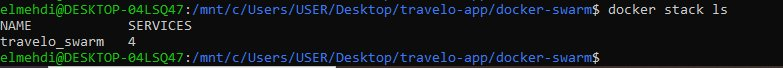
\includegraphics[width=0.95\textwidth]{./screenshots/volet1/53_docker_stack_ls_travelo_swarm_4_services.png}
    \caption{\texttt{docker stack ls} : stack travelo\_swarm avec 4 services}
\end{figure}

\subsubsection{Liste des services déployés}

\begin{lstlisting}[language=bash]
docker service ls
\end{lstlisting}

\begin{figure}[H]
    \centering
    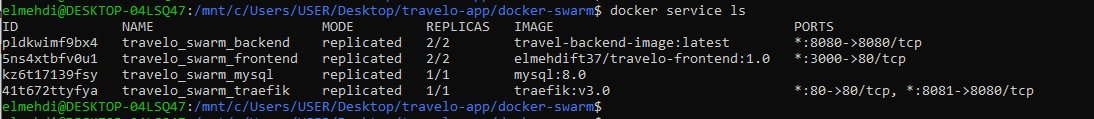
\includegraphics[width=0.95\textwidth]{./screenshots/volet1/54_docker_service_ls_backend_frontend_mysql_traefik_replicas.png}
    \caption{\texttt{docker service ls} : backend (2/2 réplicas), frontend (2/2), mysql (1/1), traefik (1/1)}
\end{figure}



\subsection{16. Restart Policy}

La politique de redémarrage \texttt{condition: on-failure} est configurée pour chaque service dans la section \texttt{deploy.restart\_policy} du fichier docker-compose.yml. Docker Swarm redémarre automatiquement les tâches défaillantes sans intervention manuelle.



\subsection{17. Accès avec Reverse Proxy Traefik}

Traefik v3.0 est configuré comme reverse proxy dans le fichier Swarm. Il écoute sur le port 80 (trafic HTTP) et expose son dashboard sur le port 8081. Le socket Docker est monté pour permettre à Traefik de découvrir les services automatiquement.

\textbf{Configuration Traefik :}

\begin{itemize}
    \item \texttt{--api.insecure=true} : Activation du dashboard Traefik sur port 8081
    \item \texttt{--providers.docker=true} : Découverte automatique des services Docker
    \item \texttt{--entrypoints.web.address=:80} : Point d'entrée HTTP sur port 80
\end{itemize}



\subsection{18. Vérification du fonctionnement du cluster}

L'application est accessible sur localhost:3000 et tous les services Swarm sont en état "Running" avec leurs réplicas opérationnels.

\begin{figure}[H]
    \centering
    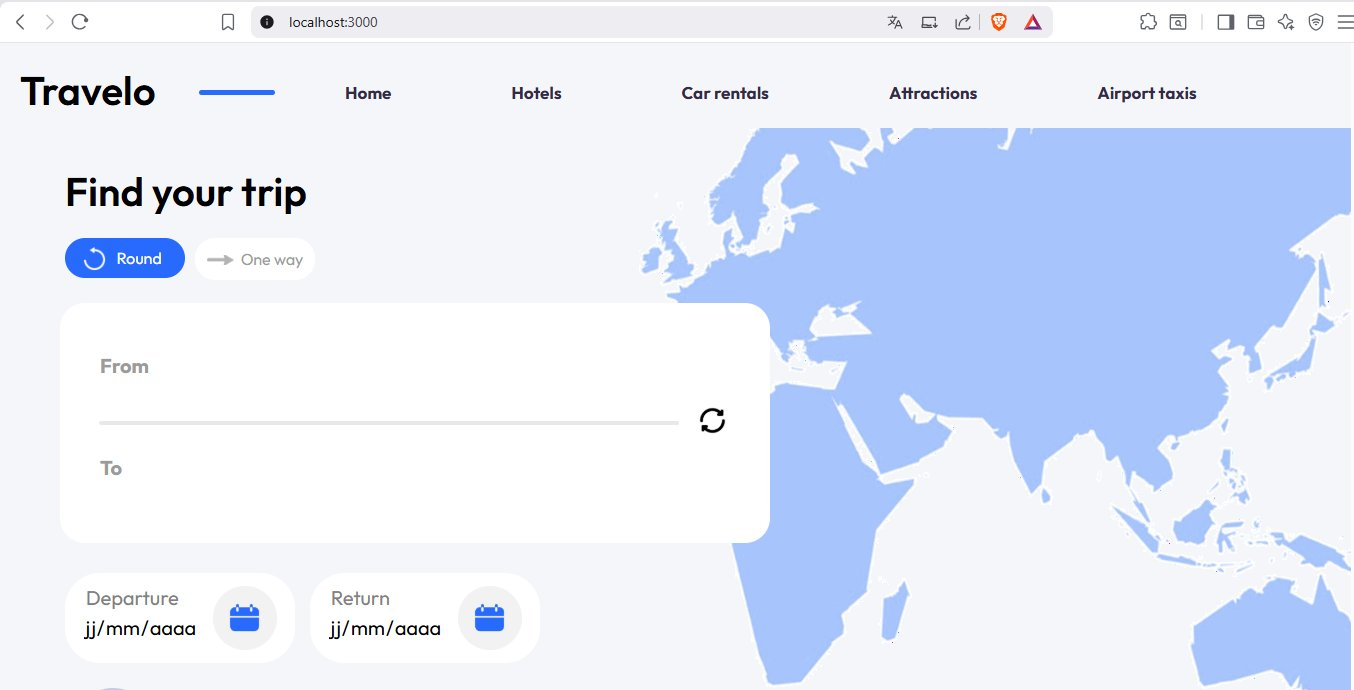
\includegraphics[width=0.95\textwidth]{./screenshots/volet1/55_travelo_accessible_localhost_3000_docker_swarm.png}
    \caption{Application Travelo accessible sur localhost:3000 via Docker Swarm}
\end{figure}

\subsubsection{État détaillé des tâches par service}

\begin{lstlisting}[language=bash]
docker service ps travelo_swarm_backend
docker service ps travelo_swarm_frontend
docker service ps travelo_swarm_mysql
\end{lstlisting}

\begin{figure}[H]
    \centering
    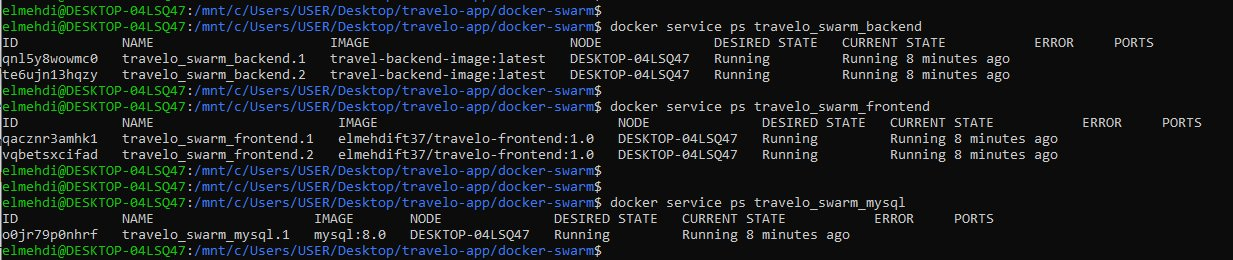
\includegraphics[width=0.95\textwidth]{./screenshots/volet1/56_docker_service_ps_backend_frontend_mysql_running.png}
    \caption{\texttt{docker service ps} : backend (2 tâches Running), frontend (2 tâches Running), mysql (1 tâche Running)}
\end{figure}



\subsection{Conclusion}

Le Volet 1 du projet a permis de conteneuriser et déployer avec succès l'application Travelo selon plusieurs modalités :

\begin{itemize}
    \item \textbf{Conteneurisation individuelle avec Docker} (réseau bridge, volumes, multi-stage builds, scan Trivy)
    \item \textbf{Déploiement orchestré via Docker Compose} (gestion des dépendances, restart policy)
    \item \textbf{Publication sur Docker Hub} (registre public) et sur un \textbf{registre privé local} (registry:2 + UI)
    \item \textbf{Redéploiement depuis le registre privé} avec Docker Compose
    \item \textbf{Bonus : Déploiement en cluster Docker Swarm} avec réplicas (haute disponibilité), limites de ressources, restart policy et reverse proxy Traefik
\end{itemize}

L'application est pleinement opérationnelle dans toutes ces configurations, comme attesté par les captures d'écran du navigateur (localhost:3000).



*Page 21 / 21*
\FloatBarrier


\section{Volet 2 : Déploiement et orchestration Kubernetes}

\subsection{Préparation de l'environnement}

Le cluster local a été créé avec \textbf{Minikube}. Ce choix est adapté au projet car Minikube fournit un environnement Kubernetes complet sur une machine locale, avec le support des objets nécessaires : Deployments, StatefulSets, Services, Ingress, ResourceQuotas, RBAC et métriques.

Les add-ons \texttt{ingress} et \texttt{metrics-server} ont été activés afin de permettre l'accès HTTP externe et la collecte de métriques CPU/RAM.

\begin{figure}[H]
    \centering
    \includesvg[width=\textwidth]{./screenshots/generated/01-minikube-status.svg}
    \caption{Statut du cluster Minikube}
\end{figure}

\begin{figure}[H]
    \centering
    \includesvg[width=\textwidth]{./screenshots/generated/02-kubectl-nodes.svg}
    \caption{Noeud Kubernetes local prêt}
\end{figure}

\subsection{Namespace travelo}

Toutes les ressources applicatives sont placées dans un namespace dédié nommé \texttt{travelo}. Cette isolation simplifie la lecture des ressources, l'application des quotas, les règles RBAC et le filtrage des métriques/logs dans les outils d'observabilité.

\begin{lstlisting}[language=bash, caption={Déploiement des manifestes Kubernetes}]
kubectl apply -k k8s/base
\end{lstlisting}

\begin{figure}[H]
    \centering
    \includesvg[width=\textwidth]{./screenshots/generated/03-namespace.svg}
    \caption{Namespace travelo créé}
\end{figure}

\subsection{Configuration et secrets}

La configuration est séparée en deux objets Kubernetes :
\begin{itemize}
    \item \textbf{ConfigMap \texttt{travelo-config}} : nom de la base, utilisateur MySQL, URL JDBC, paramètres JPA.
    \item \textbf{Secret \texttt{travelo-secret}} : mots de passe MySQL et mot de passe de la datasource Spring.
\end{itemize}

Cette séparation évite de coder les paramètres directement dans les images Docker ou dans le code applicatif. Les Deployments consomment ensuite ces valeurs via \texttt{configMapKeyRef} et \texttt{secretKeyRef}.

\begin{figure}[H]
    \centering
    \includesvg[width=\textwidth]{./screenshots/generated/06-configmaps-secrets.svg}
    \caption{ConfigMap et Secret du namespace travelo}
\end{figure}

\subsection{Base de données MySQL avec StatefulSet}

La base de données est déployée avec un \texttt{StatefulSet}, car elle doit conserver son identité et ses données. Le service \texttt{mysql} est un service headless, ce qui donne une identité réseau stable au pod \texttt{mysql-0}. Les données sont stockées dans un \texttt{PersistentVolumeClaim} monté dans \texttt{/var/lib/mysql}.

Les principaux choix techniques sont :
\begin{itemize}
    \item image \texttt{mysql:8.0};
    \item un réplica, adapté à un environnement local Minikube;
    \item stockage persistant de \texttt{2Gi};
    \item requests/limits : \texttt{250m/1 CPU} et \texttt{512Mi/1Gi};
    \item probes \texttt{startup}, \texttt{readiness} et \texttt{liveness} basées sur \texttt{mysqladmin ping}.
\end{itemize}

\begin{figure}[H]
    \centering
    \includesvg[width=\textwidth]{./screenshots/generated/16-mysql-probes.svg}
    \caption{MySQL : état du pod, PVC, ressources et probes}
\end{figure}

\subsection{Backend Spring Boot avec Deployment}

Le backend est stateless : il ne stocke pas d'état local durable et peut donc être répliqué horizontalement. Il est déployé avec un \texttt{Deployment} de \textbf{2 réplicas}, exposé par un service \texttt{ClusterIP} nommé \texttt{backend} sur le port \texttt{8080}.

Le déploiement utilise une stratégie \texttt{RollingUpdate} avec \texttt{maxUnavailable: 0} et \texttt{maxSurge: 1}. Cela permet de mettre à jour le backend sans retirer tous les pods disponibles en même temps. Les probes HTTP vérifient l'endpoint \texttt{/api/hello}.

\begin{figure}[H]
    \centering
    \includesvg[width=\textwidth]{./screenshots/generated/14-backend-probes.svg}
    \caption{Backend : 2 réplicas, ressources et probes HTTP}
\end{figure}

\subsection{Frontend React avec Deployment}

Le frontend est également stateless et déployé avec un \texttt{Deployment} de \textbf{2 réplicas}. Il est exposé en interne par le service \texttt{frontend} sur le port \texttt{80}. Les probes HTTP vérifient la route \texttt{/}, servie par Nginx.

\begin{figure}[H]
    \centering
    \includesvg[width=\textwidth]{./screenshots/generated/15-frontend-probes.svg}
    \caption{Frontend : 2 réplicas, ressources et probes HTTP}
\end{figure}

\subsection{Réseau interne et services}

Les communications internes s'appuient sur les services Kubernetes :
\begin{itemize}
    \item \texttt{mysql} : service headless pour le StatefulSet MySQL;
    \item \texttt{backend} : service \texttt{ClusterIP} vers les pods Spring Boot;
    \item \texttt{frontend} : service \texttt{ClusterIP} vers les pods Nginx/React.
\end{itemize}

Le backend accède à MySQL avec l'URL JDBC \texttt{jdbc:mysql://mysql:3306/travelo\_db}. Kubernetes résout automatiquement ce nom grâce au DNS interne du namespace.

\begin{figure}[H]
    \centering
    \includesvg[width=\textwidth]{./screenshots/generated/05-workloads-services-ingress-pdb.svg}
    \caption{Deployments, StatefulSet, Services, Ingress et PDB}
\end{figure}

\subsection{Scalabilité et état des pods}

Le frontend et le backend disposent chacun de 2 réplicas, conformément au cahier des charges. La capture suivante montre les pods en état \texttt{Running}, leur readiness et leur placement sur le noeud Minikube.

\begin{figure}[H]
    \centering
    \includesvg[width=\textwidth]{./screenshots/generated/04-pods-wide.svg}
    \caption{Pods Travelo en exécution}
\end{figure}

\subsection{ResourceQuota et requests/limits}

Un \texttt{ResourceQuota} limite la consommation totale du namespace \texttt{travelo} :
\begin{itemize}
    \item requests : \texttt{2 CPU} et \texttt{2Gi};
    \item limits : \texttt{4 CPU} et \texttt{4Gi};
    \item nombre maximal de pods, services et PVC.
\end{itemize}

Chaque composant définit aussi ses propres \texttt{requests} et \texttt{limits}. Cela rend le scheduling plus prévisible et évite qu'un composant consomme toutes les ressources du cluster.

\begin{figure}[H]
    \centering
    \includesvg[width=\textwidth]{./screenshots/generated/07-resource-quota.svg}
    \caption{ResourceQuota appliqué au namespace travelo}
\end{figure}

\subsection{PodDisruptionBudget}

Deux \texttt{PodDisruptionBudget} sont configurés : un pour le frontend et un pour le backend. Chaque PDB impose \texttt{minAvailable: 1}. Ainsi, lors d'une maintenance volontaire ou d'un drain de noeud, Kubernetes doit conserver au moins un pod disponible pour chaque partie stateless.

\begin{figure}[H]
    \centering
    \includesvg[width=\textwidth]{./screenshots/generated/05-workloads-services-ingress-pdb.svg}
    \caption{PDB frontend-pdb et backend-pdb}
\end{figure}

\subsection{Sécurité RBAC}

Le projet applique le principe du moindre privilège avec :
\begin{itemize}
    \item un \texttt{ServiceAccount} nommé \texttt{travelo-deployer};
    \item un \texttt{Role} limité à la lecture des ressources utiles dans le namespace;
    \item un \texttt{RoleBinding} qui lie ce rôle au ServiceAccount.
\end{itemize}

La validation montre que ce compte peut lire les pods, mais ne peut pas les supprimer. Cette preuve est importante car elle démontre que la restriction RBAC est réellement active.

\begin{figure}[H]
    \centering
    \includesvg[width=\textwidth]{./screenshots/generated/08-rbac-can-read.svg}
    \caption{RBAC : lecture autorisée}
\end{figure}

\begin{figure}[H]
    \centering
    \includesvg[width=\textwidth]{./screenshots/generated/09-rbac-cannot-delete.svg}
    \caption{RBAC : suppression refusée}
\end{figure}

\subsection{Accès externe avec Ingress}

L'accès HTTP externe est configuré avec l'Ingress Controller Nginx de Minikube. Deux noms de domaine locaux sont définis :
\begin{itemize}
    \item \texttt{frontend.exam.local} vers le service \texttt{frontend:80};
    \item \texttt{backend.exam.local} vers le service \texttt{backend:8080}.
\end{itemize}

La commande \texttt{kubectl describe ingress} confirme l'adresse Minikube, les règles de routage et les endpoints backend associés.

\begin{figure}[H]
    \centering
    \includesvg[width=\textwidth]{./screenshots/generated/10-ingress.svg}
    \caption{Ingress travelo-ingress et règles de routage}
\end{figure}

Des tests HTTP et navigateur ont ensuite validé que le frontend et le backend répondent correctement depuis l'environnement Kubernetes.

\begin{figure}[H]
    \centering
    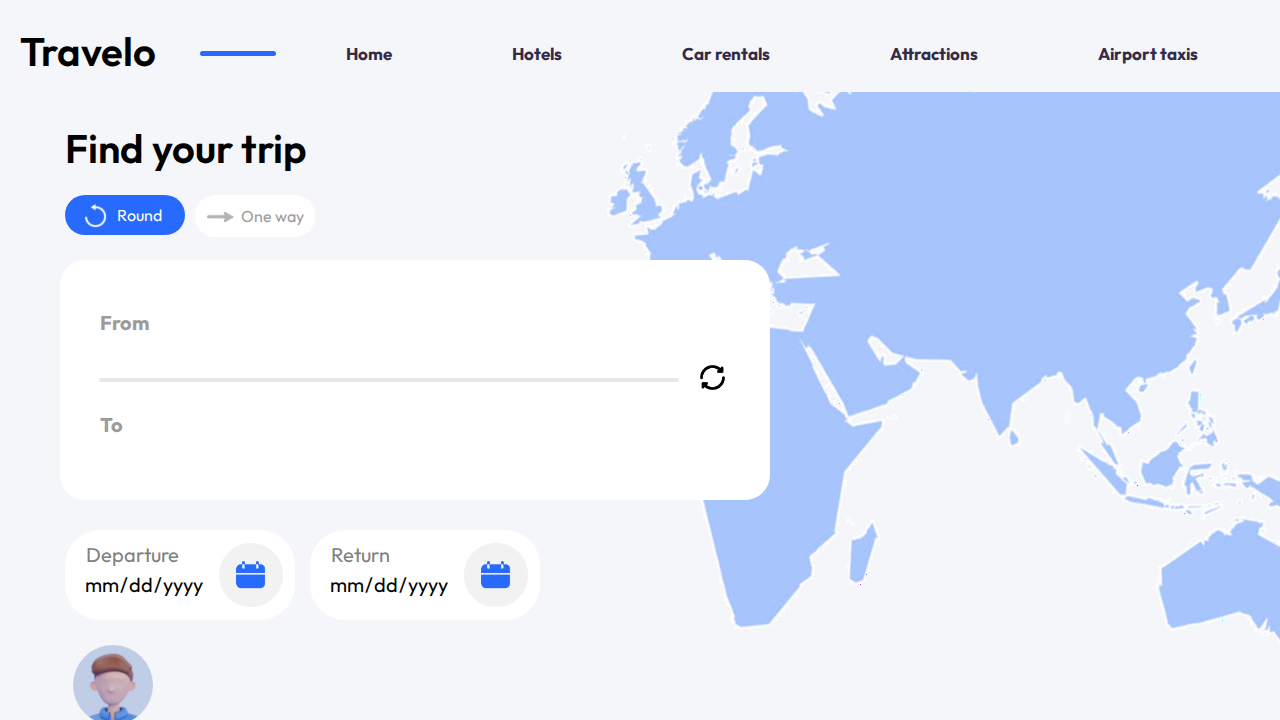
\includegraphics[width=0.92\textwidth]{./screenshots/generated/30-frontend-browser.png}
    \caption{Interface Travelo accessible depuis le navigateur}
\end{figure}

\begin{figure}[H]
    \centering
    
\includegraphics[width=0.92\textwidth]{./screenshots/generated/31-backend-browser.png}
    \caption{Endpoint backend \texttt{/api/hello} accessible depuis le navigateur}
\end{figure}

\begin{figure}[H]
    \centering
    \includesvg[width=\textwidth]{./screenshots/generated/17-frontend-http-access.svg}
    \caption{Validation HTTP du frontend}
\end{figure}

\begin{figure}[H]
    \centering
    \includesvg[width=\textwidth]{./screenshots/generated/18-backend-http-access.svg}
    \caption{Validation HTTP du backend}
\end{figure}

\subsection{Validation par kubectl et métriques}

La validation opérationnelle a été réalisée avec \texttt{kubectl get}, \texttt{kubectl describe}, \texttt{kubectl logs} et \texttt{kubectl top}. Les captures suivantes montrent que les pods sont prêts, que les logs backend sont consultables et que les métriques CPU/RAM remontent correctement.

\begin{figure}[H]
    \centering
    \includesvg[width=\textwidth]{./screenshots/generated/11-backend-logs.svg}
    \caption{Logs du backend Spring Boot}
\end{figure}

\begin{figure}[H]
    \centering
    \includesvg[width=\textwidth]{./screenshots/generated/12-top-nodes.svg}
    \caption{Métriques du noeud via metrics-server}
\end{figure}

\begin{figure}[H]
    \centering
    \includesvg[width=\textwidth]{./screenshots/generated/13-top-pods.svg}
    \caption{Métriques des pods Travelo}
\end{figure}

\FloatBarrier
\section{Volet 3 : Observabilité et monitoring}

\subsection{Monitoring de l'infrastructure}

Le monitoring de l'infrastructure est assuré par le chart Helm \texttt{kube-prometheus-stack}. Il installe Prometheus, Grafana, Alertmanager, kube-state-metrics et node-exporter. Cette stack permet de superviser :
\begin{itemize}
    \item l'utilisation CPU et mémoire des noeuds;
    \item l'état des pods et leurs redémarrages;
    \item les métriques Kubernetes exposées par kube-state-metrics;
    \item les ressources système du cluster local.
\end{itemize}

\begin{figure}[H]
    \centering
    \includesvg[width=\textwidth]{./screenshots/generated/19-monitoring-pods.svg}
    \caption{Pods de la stack monitoring}
\end{figure}

\begin{figure}[H]
    \centering
    \includesvg[width=\textwidth]{./screenshots/generated/20-helm-monitoring-releases.svg}
    \caption{Releases Helm de monitoring installées}
\end{figure}

\subsection{Monitoring applicatif}

Le backend Spring Boot expose des métriques applicatives grâce à Actuator et à Micrometer Prometheus. L'endpoint \texttt{/actuator/prometheus} est découvert par Prometheus via un \texttt{ServiceMonitor}.

Le tableau de bord Grafana \textbf{Travelo Application Overview} centralise les métriques utiles : CPU par pod, mémoire par pod, redémarrages et logs associés au namespace \texttt{travelo}.

\begin{figure}[H]
    \centering
    \includesvg[width=\textwidth]{./screenshots/generated/21-servicemonitor.svg}
    \caption{ServiceMonitor du backend Travelo}
\end{figure}

\begin{figure}[H]
    \centering
    \includesvg[width=\textwidth]{./screenshots/generated/22-grafana-dashboard-configmap.svg}
    \caption{ConfigMap du dashboard Grafana Travelo}
\end{figure}

\begin{figure}[H]
    \centering
    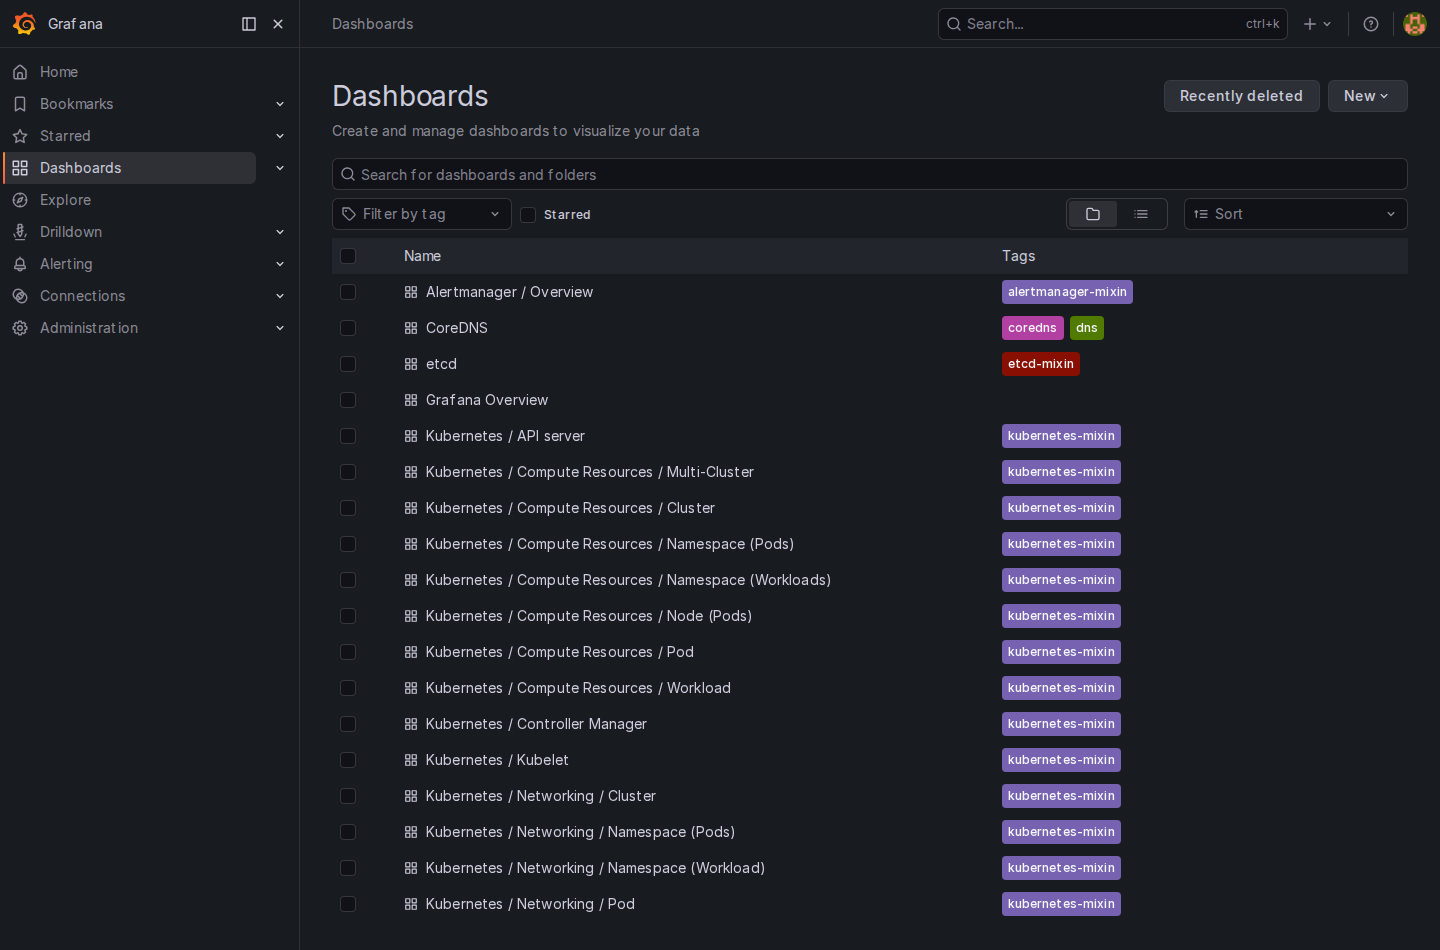
\includegraphics[width=\textwidth]{./screenshots/generated/33-grafana-dashboards-authenticated.png}
    \caption{Grafana authentifié avec les dashboards disponibles}
\end{figure}

\begin{figure}[H]
    \centering
    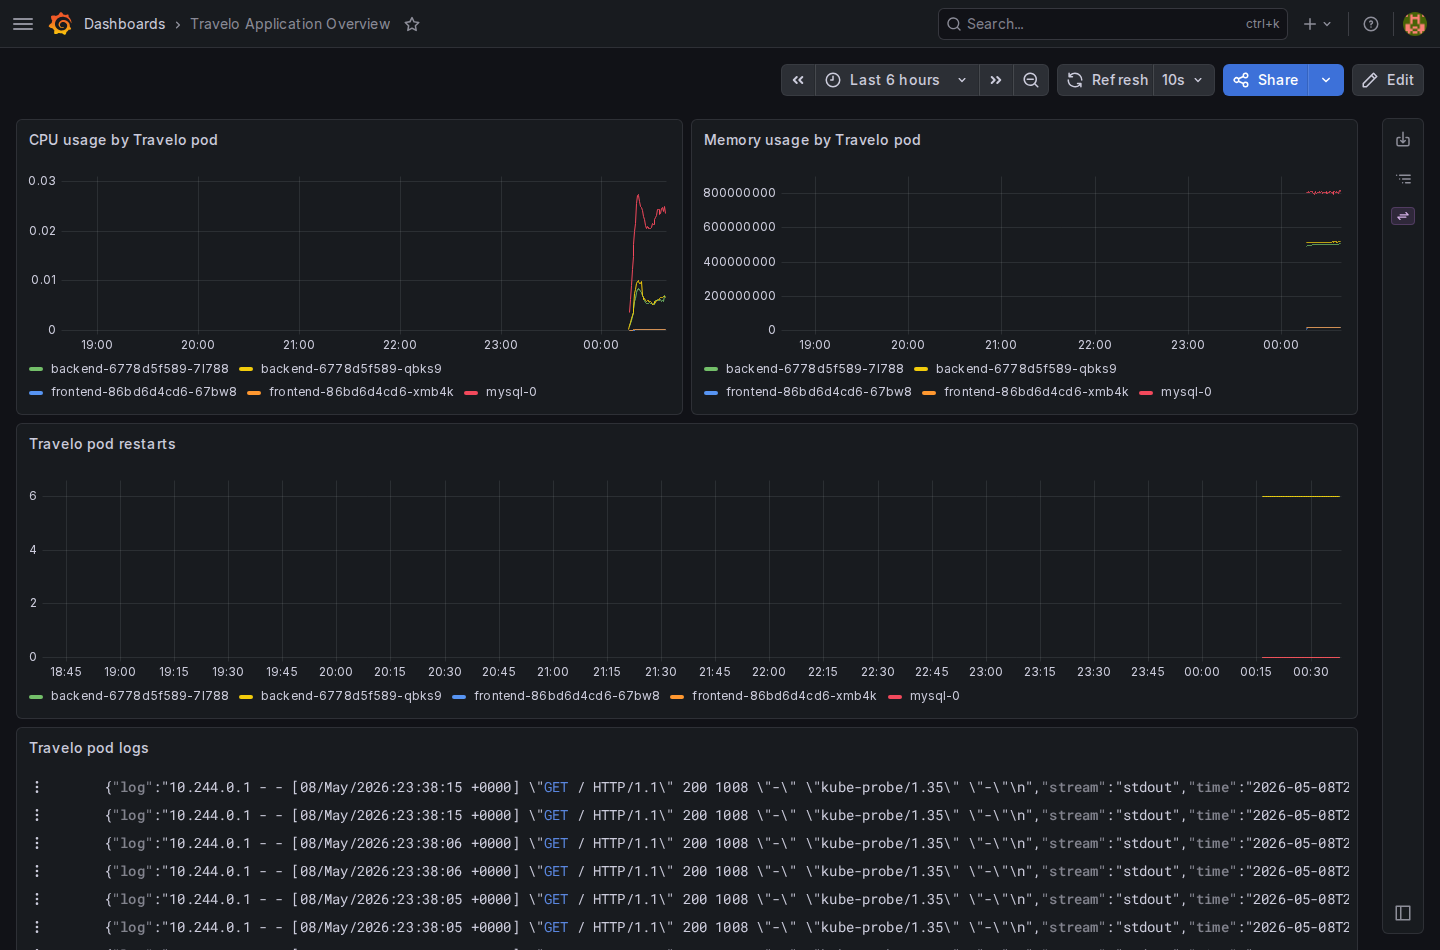
\includegraphics[width=\textwidth]{./screenshots/generated/34-grafana-travelo-dashboard.png}
    \caption{Dashboard Grafana Travelo : CPU, mémoire, redémarrages et logs}
\end{figure}

\subsection{Monitoring des logs}

La centralisation des journaux est réalisée avec \textbf{Loki} et \textbf{Promtail}. Promtail collecte les logs des pods, enrichit les entrées avec des labels Kubernetes comme \texttt{namespace}, \texttt{pod} et \texttt{container}, puis les envoie à Loki. Grafana interroge ensuite Loki avec des requêtes LogQL.

La requête principale utilisée pour l'application est :

\begin{lstlisting}[language=bash, caption={Requête LogQL pour les logs Travelo}]
{namespace="travelo"}
\end{lstlisting}

\begin{figure}[H]
    \centering
    \includesvg[width=\textwidth]{./screenshots/generated/23-loki-datasource-configmap.svg}
    \caption{Datasource Loki ajoutée à Grafana}
\end{figure}

\begin{figure}[H]
    \centering
    \includesvg[width=\textwidth]{./screenshots/generated/24-loki-promtail.svg}
    \caption{Loki et Promtail déployés dans le namespace monitoring}
\end{figure}

\begin{figure}[H]
    \centering
    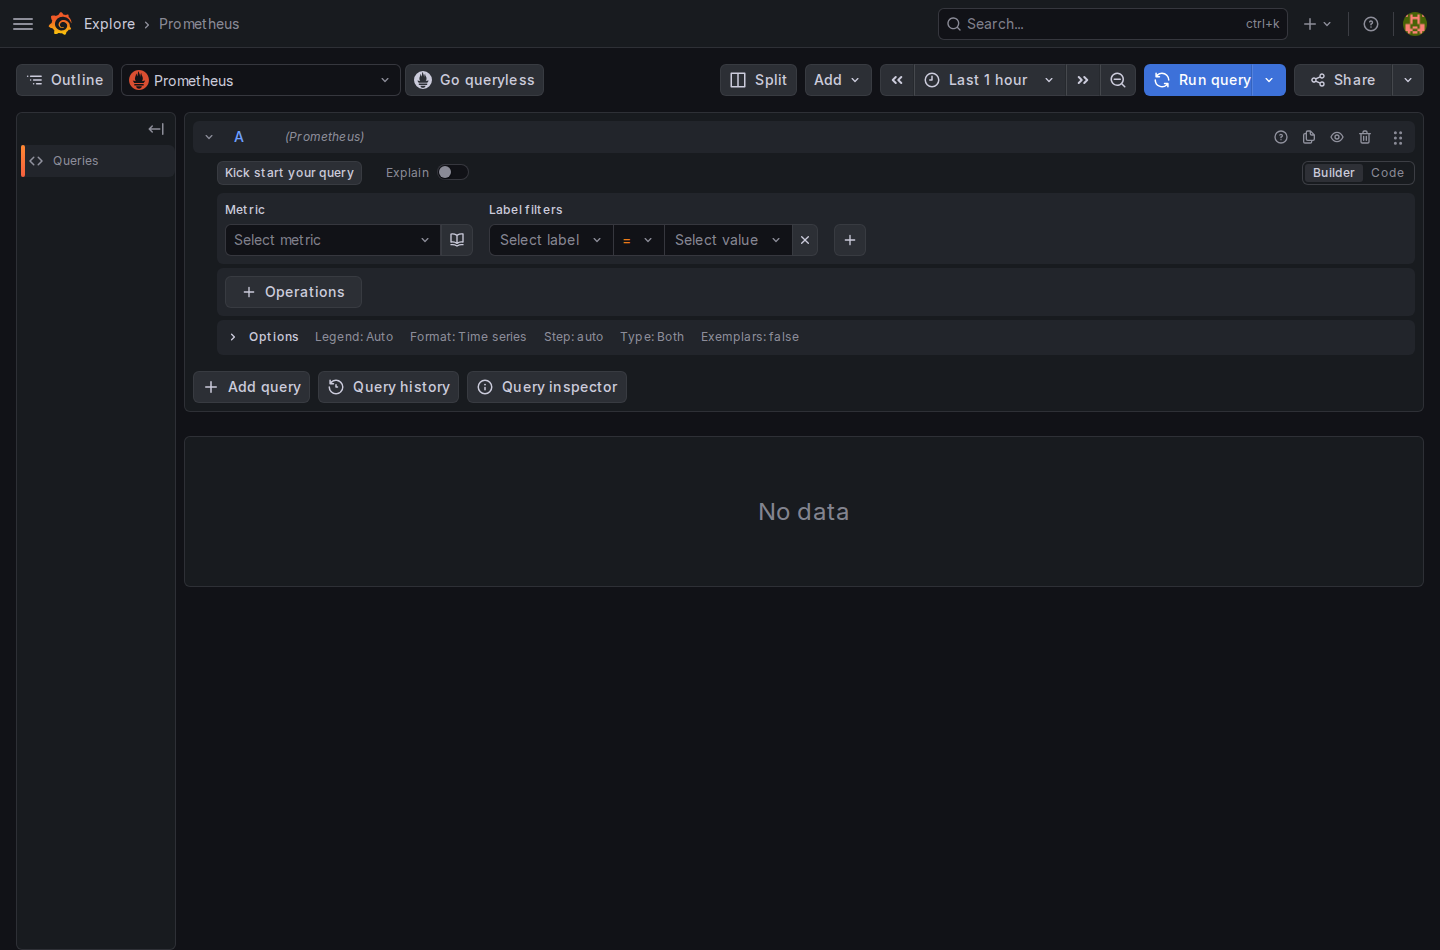
\includegraphics[width=\textwidth]{./screenshots/generated/35-grafana-explore-logs.png}
    \caption{Exploration des logs Travelo dans Grafana}
\end{figure}

\FloatBarrier
\section{Bonus réalisés}

\subsection{Skaffold}

Le fichier \texttt{skaffold.yaml} automatise le cycle de développement en construisant les images frontend/backend puis en déployant les manifestes \texttt{k8s/base}. Il permet d'utiliser :

\begin{lstlisting}[language=bash, caption={Workflow Skaffold}]
skaffold dev
skaffold run
\end{lstlisting}

\subsection{Helm Chart}

Un chart Helm complet est fourni dans \texttt{k8s/helm/travelo}. Il reprend les composants principaux de l'application et les rend paramétrables via \texttt{values.yaml} : namespace \texttt{travelo-helm}, images, réplicas, ressources, MySQL et Ingress.

\begin{lstlisting}[language=bash, caption={Déploiement Helm bonus}]
helm upgrade --install travelo k8s/helm/travelo --namespace travelo-helm --create-namespace
\end{lstlisting}

\subsection{GitOps avec Argo CD}

Le dossier \texttt{k8s/gitops/} contient un exemple de manifeste \texttt{Application} Argo CD. Après remplacement de \texttt{repoURL} par le dépôt GitHub réel, Argo CD peut synchroniser automatiquement le cluster à partir du dépôt Git.

\section{Synthèse de conformité}

\begin{table}[H]
\centering
\begin{tabular}{|p{0.45\textwidth}|p{0.42\textwidth}|}
\hline
\textbf{Exigence} & \textbf{Preuve dans le projet} \\
\hline
Conteneurisation Docker & Volet 1, Dockerfiles frontend/backend, captures \texttt{01} à \texttt{21} du dossier \texttt{screenshots/volet1} \\
\hline
Exécution locale Docker Compose & Volet 1, captures \texttt{29} à \texttt{33} \\
\hline
Publication Docker Hub et registre privé & Volet 1, captures \texttt{10}, \texttt{11}, \texttt{20}, \texttt{21}, \texttt{35} à \texttt{47} \\
\hline
Déploiement Docker Swarm bonus & Volet 1, captures \texttt{48} à \texttt{56} \\
\hline
Cluster Kubernetes local & Minikube, captures \texttt{01} et \texttt{02} \\
\hline
Namespace \texttt{travelo} & \texttt{k8s/base/00-namespace.yaml}, capture \texttt{03} \\
\hline
Deployments frontend/backend & \texttt{06-backend-deployment.yaml}, \texttt{07-frontend-deployment.yaml} \\
\hline
StatefulSet base de données & \texttt{05-mysql-statefulset.yaml} \\
\hline
Services Kubernetes & Services \texttt{mysql}, \texttt{backend}, \texttt{frontend} \\
\hline
ConfigMap et Secrets & \texttt{03-configmap.yaml}, \texttt{04-secret.yaml} \\
\hline
2 réplicas frontend/backend & Captures \texttt{04}, \texttt{14}, \texttt{15} \\
\hline
ResourceQuota et requests/limits & \texttt{01-resourcequota.yaml}, captures \texttt{07}, \texttt{14}, \texttt{15}, \texttt{16} \\
\hline
Liveness, readiness, startup probes & Captures \texttt{14}, \texttt{15}, \texttt{16} \\
\hline
PodDisruptionBudget & \texttt{08-pdb.yaml}, capture \texttt{05} \\
\hline
RBAC restreint & \texttt{02-rbac.yaml}, captures \texttt{08} et \texttt{09} \\
\hline
Ingress & \texttt{09-ingress.yaml}, capture \texttt{10} \\
\hline
Accès navigateur & Captures \texttt{30} et \texttt{31} \\
\hline
Monitoring infrastructure & \texttt{kube-prometheus-stack}, captures \texttt{19}, \texttt{20}, \texttt{34} \\
\hline
Monitoring applicatif & Actuator, Micrometer, ServiceMonitor, captures \texttt{21}, \texttt{34} \\
\hline
Monitoring logs & Loki, Promtail, captures \texttt{23}, \texttt{24}, \texttt{35} \\
\hline
Lien du dépôt Git & \url{https://github.com/ElmehdiFATAHLLAH/travelo-app.git} \\
\hline
\end{tabular}
\caption{Couverture des exigences du sujet}
\end{table}

\section{Conclusion}

Le projet Travelo couvre l'ensemble du cycle demandé. Le Volet 1 documente la conteneurisation Docker des trois composants, l'utilisation d'un réseau et d'un volume persistant, les builds multi-stage, les scans Trivy, la publication sur Docker Hub, le registre privé local, Docker Compose et le déploiement bonus avec Docker Swarm.

Le projet répond aussi aux exigences du volet Kubernetes : composants déployés dans le namespace \texttt{travelo}, Deployments pour les services stateless, StatefulSet pour MySQL, Services, ConfigMaps, Secrets, quotas, probes, PDB, RBAC et Ingress. Les captures montrent également la validation par \texttt{kubectl}, l'accès HTTP et l'accès navigateur.

Le volet observabilité est couvert par une stack complète : Prometheus et Grafana pour les métriques infrastructure/applicatives, ServiceMonitor pour le backend Spring Boot, Loki et Promtail pour les logs. Les bonus Skaffold, Helm et GitOps sont également préparés dans le dépôt, ce qui améliore la qualité DevOps globale du rendu.

\end{document}
